\let\texyear\year
\documentclass{ieeeaccess}
\let\ieeeaccessyear\year
\let\year\texyear
    \usepackage{orcidlink}
\let\year\ieeeaccessyear
\definecolor{accessblue}{RGB}{0,105,154}

\usepackage{cite}
\usepackage{amsmath,amssymb,amsfonts}
\usepackage{algorithmic}
\usepackage{graphicx}
\usepackage{textcomp}
\usepackage{makecell}

\usepackage{caption}
\usepackage{bm}
\usepackage{booktabs}
\usepackage{multirow}
\usepackage{microtype}
\usepackage{lmodern}
\usepackage{url}
\usepackage{xcolor}
\usepackage{etoolbox}
\makeatletter
\@ifundefined{if@biographyTOCentrynotmade}{\newif\if@biographyTOCentrynotmade\@biographyTOCentrynotmadetrue}{}
\@ifundefined{c@biography}{\newcounter{biography}}{}
\patchcmd{\@maketitle}{Digital Object Identifier\space\@doi}{}{}{\PackageError{aratoken}{Unable to remove unassigned DOI line}{Check the IEEE Access class version}}
\patchcmd{\appendices}{\thesectiondis{APPENDIX \Alph{section}}.}{\thesectiondis{APPENDIX \Alph{section}}}{}{\PackageError{aratoken}{Unable to remove stray appendix punctuation}{Check the IEEE Access class version}}
\patchcmd{\thebibliography}{\section*{\refname}}{\section*{\refname}\phantomsection}{}{\PackageError{aratoken}{Unable to anchor the bibliography heading}{Check the IEEE Access class version}}
\newcommand{\reviewfooters}{\def\@oddfoot{\hfil{\footerpagefont\thepage}}\let\@evenfoot\@oddfoot}
\let\accessheadings\ps@headings
\let\accesstitlepage\ps@titlepage
\def\ps@headings{\accessheadings\reviewfooters}
\def\ps@titlepage{\accesstitlepage\reviewfooters}
\pagestyle{headings}
\makeatother
\newsavebox{\fitbox}
\newcommand{\fitcolumn}[1]{\sbox{\fitbox}{#1}%
  \ifdim\wd\fitbox>\linewidth\resizebox{\linewidth}{!}{\usebox{\fitbox}}%
  \else\usebox{\fitbox}\fi}
\def\BibTeX{{\rm B\kern-.05em{\sc i\kern-.025em b}\kern-.08em
    T\kern-.1667em\lower.7ex\hbox{E}\kern-.125emX}}

\newtheorem{proposition}{Proposition}

\begin{document}
\history{}
\doi{}

\title{AraToken: Optimizing Arabic Tokenization with Normalization Pipeline and Language Extension for Qwen3}
\author{\uppercase{Mark Kashirskiy \authorrefmark{1, 2}, Artiom Lipinski \authorrefmark{3}  and Ilya Makarov\authorrefmark{4,5} (Member, IEEE)}}
\address[1]{HSE University, 101000 Moscow, Russia}
\address[2]{AI Talent Hub, ITMO University, 197101 Saint Petersburg, Russia}
\address[3]{Saint Petersburg State University, 199034 Saint Petersburg, Russia}
\address[4]{Artificial Intelligence Research Institute (AIRI), 105064 Moscow, Russia}
\address[5]{Trusted AI Center, RAS, 109004 Moscow, Russia}

\tfootnote{The work was supported by a grant, provided by the Ministry of Economic Development of the Russian Federation (agreement dated June 20, 2025 No. 139-15-2025-011, identifier 000000C313925P4G0002).}
\markboth
{Kashirskiy \headeretal: AraToken}
{Kashirskiy \headeretal: AraToken}

\corresp{Corresponding author: Mark Kashirskiy (e-mail: 353056@niuitmo.ru).}

\begin{abstract}
Arabic token fragmentation limits the text represented within a language
model's token budget. We present AraToken, an Arabic normalization and
SentencePiece Unigram tokenizer, and the Language Extension Pipeline
(LEP), which adds its vocabulary to Qwen3. AraToken uses 44.4\% fewer tokens
per word than Qwen3 on 5{,}000 commonly normalized test documents.
LEP initializes new embedding rows with a fixed average of compositional
and character-ngram analogical estimates. We evaluate 78 controlled runs
with three training seeds, two base-model sizes and explicit embedding
and transformer trainability controls. Across six comparisons at matched
nominal token budgets, LEP lowers canonical-Arabic bits per character by
0.035--0.123 relative to continued pretraining (CPT), while requiring
23--28\% more trainer runtime. The fixed mixture improves on both
components at the original 0.6B budget and at 1.7B, but its advantage over
the analogical component is unresolved at the larger 0.6B budget.
LEP achieves the highest mean accuracy on five Arabic tasks: 40.65\%,
versus 39.58\% for CPT and 39.20\% for the base, although the aggregate
accuracy differences are not statistically resolved. On two English tasks,
LEP averages 62.92\%, improving on CPT's 58.33\% while remaining below the
unadapted base's 66.65\%.
The strongest findings are consistent Arabic compression and likelihood
gains, accompanied by task-dependent accuracy gains and better English
retention than CPT under the tested adaptation policies.
\end{abstract}

\begin{keywords}
Arabic natural language processing, embedding initialization, large language models, tokenization, vocabulary extension
\end{keywords}

\titlepgskip=-15pt

\maketitle

\section{Introduction}
\label{sec:introduction}

The tokenizer decides how many tokens a language model spends on a text.
Token counts can differ substantially across languages
\cite{rust2021good, petrov2023language}. Arabic illustrates this problem.
Figure~\ref{fig:segmentation} shows how three tokenizers split the same
words. The Qwen3 tokenizer cuts \emph{their libraries} into four pieces and
the borrowing \emph{technology} into four more, while AraToken, the tokenizer
we present here, keeps the stem of the first word intact and the second word
whole. More tokens leave less text in a fixed-length token window;
training and inference costs also depend on the model and execution setup.\footnote{AI assistance: OpenAI Codex~\cite{openaicodex2026}; see Acknowledgment.}

Arabic is hard to tokenize for two reasons. First, one word often carries a
conjunction, a preposition, a stem and a possessive pronoun, all written
without spaces \cite{habash2010introduction}. Second, the same word can be
spelled in several ways: Alif has four common variants, diacritics are
optional, the decorative Tatweel stretches words, and writers mix
Arabic-Indic and Western digits and punctuation
\cite{numbencheval, yagi2024arabic}. A tokenizer that ignores these
properties spends its vocabulary on spelling variants of the same word.

Two lines of work address the problem. The first trains an Arabic tokenizer
together with a new model, as in AraBERT \cite{antoun2020arabert} and the
Arabic large language model (LLM) Jais \cite{sengupta2023jais}. The second extends the vocabulary of
an existing model with Arabic tokens and continues training
\cite{kuwain_2025, arallama_2024, rightnow_2026}. This reuses the pretrained
model and requires an initialization for the added embeddings.
Mean sub-token initialization averages the embeddings of the pieces produced
by the old tokenizer \cite{tejaswi2024design}. WECHSEL
\cite{minixhofer2022wechsel} and FOCUS \cite{dobler2023focus} instead use
similarity in auxiliary embedding spaces. We study a fixed average of the
sub-token estimate and a character-overlap estimate for Arabic vocabulary
extension.

We train AraToken, an Arabic tokenizer with an explicit normalization
pipeline, and add its vocabulary to Qwen3 \cite{qwen3technicalreport}
with the Language Extension Pipeline (LEP). LEP trains the new embedding
rows and selected transformer layers. We compare mean sub-token
initialization with a character-overlap initializer and their fixed average.
The character-overlap initializer is a lexical proxy rather than an
implementation of WECHSEL or FOCUS. We use bits per character (BPC) to
compare models on the same declared character spans, with the initializer
and trainable parameters identified for each configuration.

Our contributions are as follows:
\begin{itemize}
\item We present AraToken, a SentencePiece Unigram tokenizer with an Arabic
normalization pipeline. On the normalized held-out sample, the full tokenizer
needs 44.4\% fewer tokens per word than Qwen3, and the pruned tokenizer needs
30.1\% fewer than AraBERT at a smaller vocabulary size
(Sections~\ref{sec:normalization}, \ref{sec:tokenizer_training},
\ref{sec:res_tokenizers} and~\ref{sec:res_pruning}).
\item We present LEP, which adds the AraToken vocabulary to Qwen3 and supports
comparisons between explicitly specified initialization and adaptation
configurations (Sections~\ref{sec:lep} and~\ref{sec:res_lep}).
\item We derive the expected squared distance of the sub-token mean from the
donor mean under stated moment assumptions, and characterize the squared
error of a fixed average relative to a reference row. We compare the
component initializers and their average empirically
(Sections~\ref{sec:init} and~\ref{sec:res_init}).
\item We describe a cross-vocabulary evaluation protocol and release
our tokenizer, training code, data splits and model checkpoints
(Section~\ref{sec:metrics}; Appendices~\ref{app:protocol} and~\ref{app:tasks};
the \hyperref[sec:availability]{Data and code availability statement}).
\end{itemize}

The rest of the paper is organized as follows. Section~\ref{sec:related}
reviews related work. Section~\ref{sec:methodology} describes AraToken and
LEP. Section~\ref{sec:experiments} describes the experimental setup, and
Section~\ref{sec:results} reports the results.
Section~\ref{sec:discussion} discusses them, and Section~\ref{sec:conclusion}
concludes the paper. The appendices give details of the evaluation protocol
and further experiments.

\begin{figure*}[t]
\centering
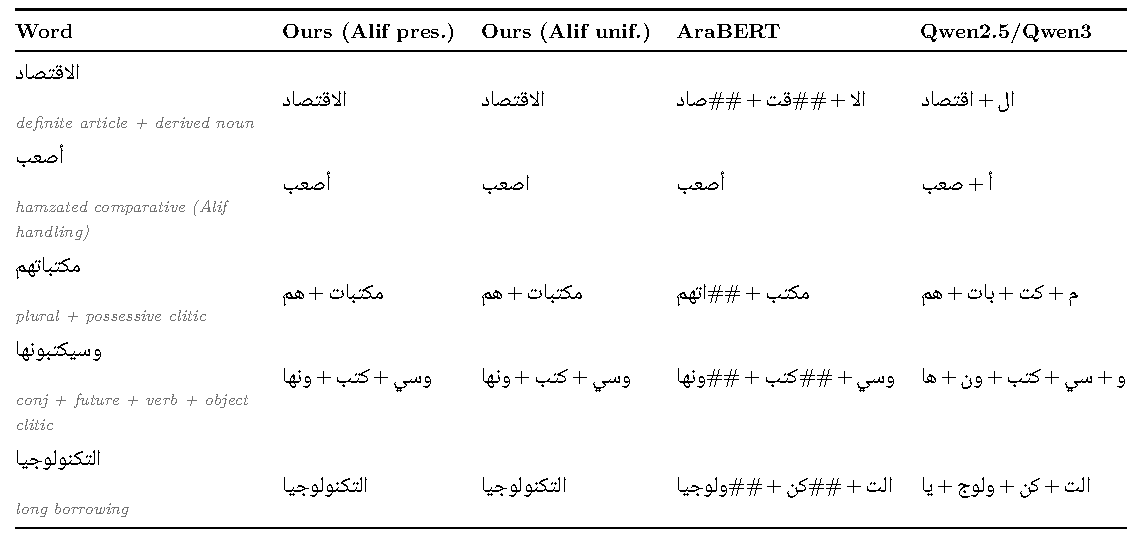
\includegraphics[width=\textwidth]{figures/segmentation_examples.pdf}
\caption{Segmentation of the same Arabic words by AraToken (ours) and two other tokenizers, each
after its own normalization; pieces are joined with ``+''. AraToken splits
\emph{their libraries} into stem and possessive clitic, where AraBERT breaks
the stem and Qwen3 produces four pieces. AraToken keeps the borrowing
\emph{technology} whole, where AraBERT needs three pieces and Qwen3 four.}
\label{fig:segmentation}
\end{figure*}

\begin{figure}[t]
\centering
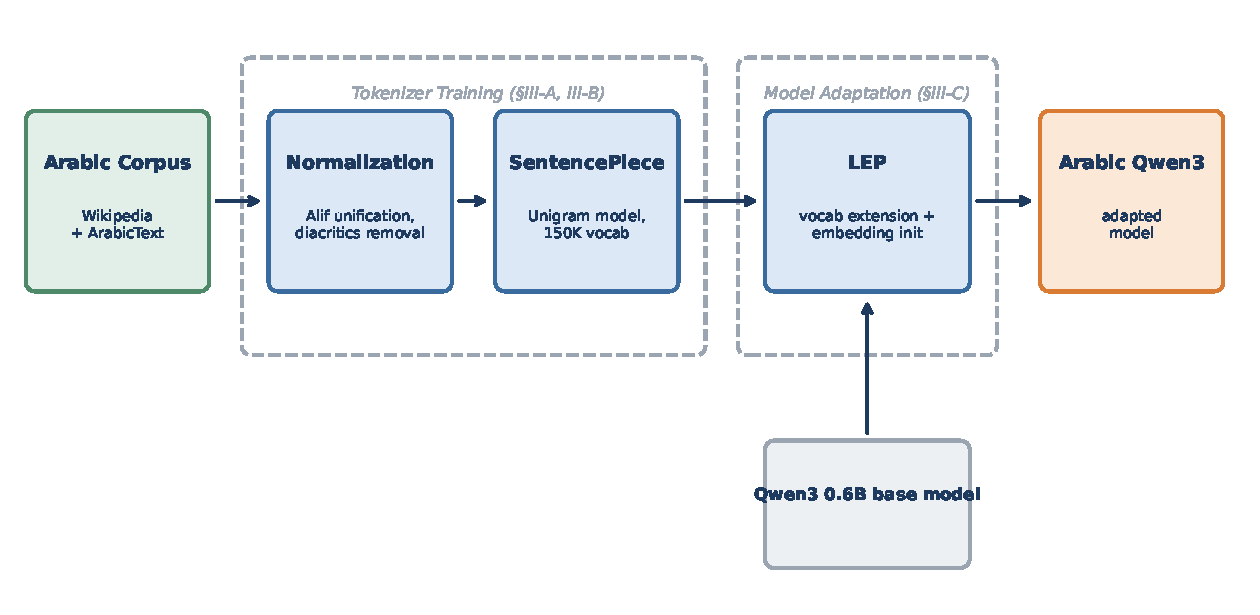
\includegraphics[width=\columnwidth]{figures/overview_pipeline.pdf}
\caption{Overview of AraToken and LEP (ours). Arabic text passes through the
normalization pipeline, a SentencePiece Unigram tokenizer is trained on the
normalized corpus, and LEP adds its vocabulary to Qwen3. NFKC denotes Unicode Normalization Form KC.}
\label{fig:overview}
\end{figure}

\section{Related Work}
\label{sec:related}

We review subword tokenization, Arabic language models, and vocabulary
extension with embedding initialization.\footnote{AI assistance: OpenAI Codex~\cite{openaicodex2026}; see Acknowledgment.}

\subsection{Subword tokenization}

Most LLMs use subword tokenizers, which trade vocabulary size against sequence
length. Byte Pair Encoding (BPE) \cite{sennrich2016neural} merges the most
frequent pair of symbols until the vocabulary reaches its target size.
WordPiece \cite{schuster2012japanese} chooses each merge by likelihood. The
Unigram model \cite{kudo2018subword} starts from a large vocabulary and
removes the pieces that contribute least to the likelihood of the corpus.
SentencePiece \cite{kudo2018sentencepiece} implements BPE and Unigram
directly on raw text, which suits languages where whitespace does not mark
morpheme boundaries, and studies of morphologically rich languages report
better compression for Unigram than for BPE \cite{dominance_unigram_2025}.
Tokenizers built for English encode other languages at a higher cost
\cite{rust2021good}, and the same text can need several times as many tokens
in some languages as in English \cite{petrov2023language}. We measure this
cost for Arabic on held-out text, distinguishing common external
normalization from each tokenizer's internal preprocessing.

\subsection{Arabic natural language processing and language models}

Arabic natural language processing (NLP) has long dealt with rich morphology and dialectal variation
\cite{darwish2021panoramic}. CAMeL Tools \cite{obeid2020camel} provides
morphological analysis and orthographic normalization for Arabic. AraBERT
\cite{antoun2020arabert}, AraBART \cite{kamal2021arabart} and AraT5
\cite{nagoudi2022arat5} were pretrained with their own Arabic tokenizers, and
recent Arabic LLMs such as Jais \cite{sengupta2023jais}, AceGPT
\cite{huang2023acegpt} and ALLaM \cite{bari2025allam} reach strong results on
Arabic benchmarks after large-scale training on Arabic and English text. Two
recent reports discuss tokenizer design and vocabulary adaptation for Arabic
\cite{tahakom_2025, kuwain_2025}. AraToken is designed to supply vocabulary
for adapting an existing model; the cost of that adaptation must be measured
for its particular training configuration.

\subsection{Vocabulary extension and embedding initialization}

Vocabulary extension adds tokens of a new language to a pretrained model and
continues training. Artetxe et al.\ \cite{artetxe2020cross} show that a frozen
transformer body transfers to a new language when only the embedding matrix
is relearned. BLOOM+1 \cite{yong2023bloom} compares continued pretraining with
adapter methods such as MAD-X \cite{pfeiffer2020mad}, and Zhao et al.\
\cite{zhao2024llama} adapt LLaMA to Chinese with less than 1\% of its
pretraining data. For Arabic, Kuwain \cite{kuwain_2025} adds about 26K tokens
to TinyLlama, AraLLaMA \cite{arallama_2024} expands the vocabulary in stages,
and RightNow-Arabic \cite{rightnow_2026} adds 27{,}032 tokens to
Qwen2.5-0.5B and trains on 504M Arabic tokens.

Each added token needs an initial embedding. Mean sub-token initialization
averages the embeddings of the pieces produced by the old tokenizer
\cite{tejaswi2024design}. WECHSEL \cite{minixhofer2022wechsel} and FOCUS
\cite{dobler2023focus} use auxiliary embedding spaces to construct
similarity-weighted estimates. VocADT \cite{han_vocadt_2025} learns new rows
with adapters. Hewitt \cite{hewitt2021initializing} analyzes how added output
rows change the next-token distribution; their logits relative to the
original partition function matter, so a small row norm alone does not
ensure a small change. Downey et al.\ \cite{downey2023embedding} study the
structure of the initialized matrix, and Joshi et al.\
\cite{joshi2026beyond} compare initialization choices for Hindi.
Yamaguchi et al.\ \cite{yamaguchi2026expand} examine their dependence on the
target-language budget. Tejaswi et al.\ \cite{tejaswi2024design} evaluate
constituent-token averaging, whereas the Mean baseline in Mundra et al.\
\cite{mundra2024empirical} averages the original vocabulary embeddings.
These are different initialization rules. Our comparison concerns a
character-overlap proxy and its fixed average with the constituent estimate,
not the original semantic-space WECHSEL and FOCUS methods. We state the
condition under which this average reduces squared error relative to both
components; its effect on language-model loss is an empirical question.

\section{Methodology}
\label{sec:methodology}

AraToken reduces the number of tokens that Arabic text costs, and LEP brings
its vocabulary into a pretrained model without pretraining from scratch.
Figure~\ref{fig:overview} shows the whole pipeline. This section describes
the normalization pipeline, the tokenizer and the three steps of LEP.\footnote{AI assistance: OpenAI Codex~\cite{openaicodex2026}; see Acknowledgment.}

\subsection{Arabic normalization pipeline}
\label{sec:normalization}

Web Arabic writes the same word in several ways, and a tokenizer trained on
raw text learns a separate piece for each spelling. The normalization
pipeline removes this variation before the tokenizer sees the text. We
implement it as a normalizer of the HuggingFace Tokenizers library
\cite{moi2023tokenizers}, so the same rules apply during training and at
inference time. The pipeline applies Unicode Normalization Form KC (NFKC), removes Tatweel
(U+0640), maps Arabic-Indic digits (U+0660--U+0669) to Western digits, and
maps the Arabic comma, semicolon and question mark (U+060C, U+061B, U+061F)
to their Latin forms. It removes diacritics by default, and a second mode
keeps them for tasks that need vocalized text. Table~\ref{tab:normalization}
lists the rules, and Figure~\ref{fig:normalization} shows their effect on
sample text.

The pipeline can also unify the four Alif variants (U+0622, U+0623, U+0625,
U+0671) into bare Alif (U+0627), as many Arabic toolkits do
\cite{obeid2020camel, habash2010introduction}. We keep the variants by
default to retain these orthographic distinctions; Alif unification is an
optional additional mapping. The rules apply to the whole input string,
including Latin lowercasing. For example, \texttt{AI} followed by a space
and Arabic-Indic digits U+0661 and U+0662 becomes \texttt{ai 12} under the
released normalizer. Retaining the original token IDs therefore does not
preserve case or guarantee a byte-for-byte round trip for mixed-script text.

\begin{table}[t]
\centering
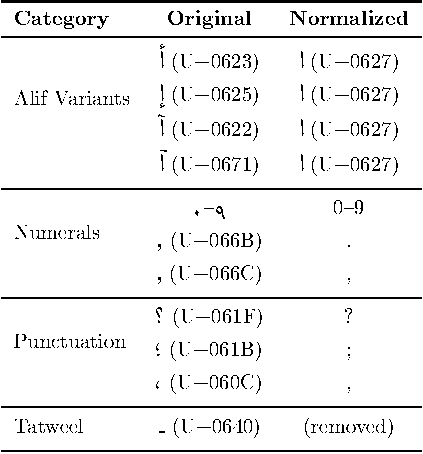
\includegraphics[width=0.75\columnwidth]{figures/normalization_table.pdf}
\caption{Character rules of the AraToken normalization pipeline (ours). Alif unification is
available as an option and is off by default.}
\label{tab:normalization}
\end{table}

\begin{figure}[t]
\centering
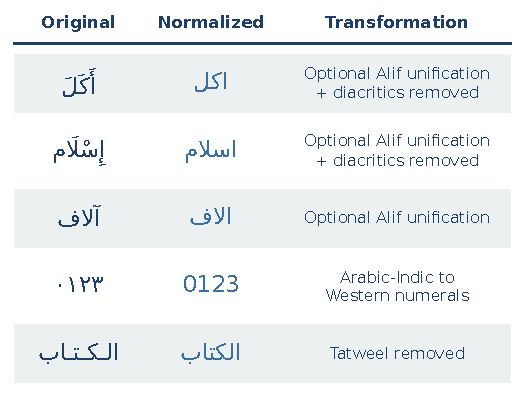
\includegraphics[width=\columnwidth]{figures/normalization_examples.pdf}
\caption{Sample text before and after AraToken normalization (ours). The first three rows
illustrate optional Alif unification; the first two also remove diacritics.}
\label{fig:normalization}
\end{figure}

\subsection{Tokenizer training}
\label{sec:tokenizer_training}

We train AraToken with the SentencePiece Unigram algorithm
\cite{kudo2018sentencepiece, kudo2018subword} on the \texttt{tok-train}
split of our corpus (Section~\ref{sec:data}): 159{,}826 documents with about
480M characters from the Arabic part of FineWeb2-HQ \cite{fineweb2hq_2025}.
We chose Unigram after comparing it with BPE and WordPiece under every
preprocessing configuration (Section~\ref{sec:res_algorithms}). The target
vocabulary has 150{,}000 pieces, close to the 151{,}643 regular tokens of
Qwen3. We also evaluate a separate SentencePiece variant with byte fallback,
which represents otherwise unsupported characters using the 8-bit Unicode Transformation Format (UTF-8). The
extended Qwen tokenizer retains its base byte-level coverage; the standalone
Unigram and byte-fallback variants are distinguished in the measurements.

A 150K vocabulary adds many embedding rows. For tighter memory budgets we
prune the vocabulary by corpus coverage: we keep the most frequent pieces
that together cover 99\% or 95\% of the tokens of the training corpus. This
gives vocabularies of 109{,}844 and 60{,}149 pieces
(Section~\ref{sec:res_pruning}).

\subsection{Language Extension Pipeline}
\label{sec:lep}

LEP adds the AraToken vocabulary to Qwen3 in three steps. It extends the
vocabulary, initializes the new embedding rows, and trains the new rows
together with the top transformer layers (Figure~\ref{fig:lep_architecture}).

\begin{figure}[t]
\centering
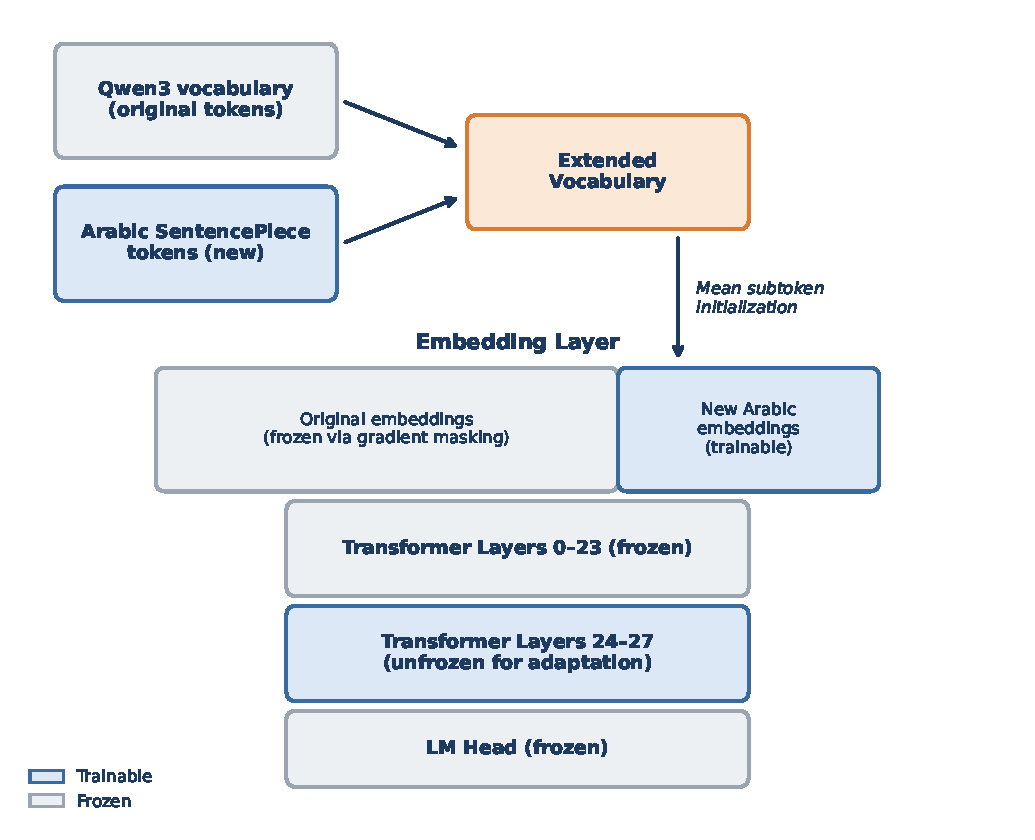
\includegraphics[width=\columnwidth]{figures/lep_architecture.pdf}
\caption{The Language Extension Pipeline (ours). New Arabic tokens are appended to
the Qwen3 vocabulary and their embedding rows are initialized. During
training, gradient masking keeps the original rows fixed, and only the new
rows and the last four transformer layers are updated. LM denotes language model.}
\label{fig:lep_architecture}
\end{figure}

\subsubsection{Vocabulary extension}

Let $\mathcal{T}_{\mathrm{ar}}$ be AraToken and $\mathcal{T}_{\mathrm{qwen}}$
the Qwen3 tokenizer. We take every piece of $\mathcal{T}_{\mathrm{ar}}$ that
is not in $\mathcal{T}_{\mathrm{qwen}}$ and drop the pieces that contain Latin
or Cyrillic letters, bare digits or punctuation, which Qwen3 already encodes
well. The Qwen3-0.6B tokenizer has 151{,}669 token IDs, whereas its embedding
matrix has 151{,}936 rows. The extended tokenizer has 282{,}826 IDs:
131{,}157 new IDs reuse 267 padded positions and require 130{,}890 appended
rows. In the initialization formulas, $n$ denotes the original tokenizer
size, $M$ the embedding matrix, and $d=1024$ the embedding dimension.
Qwen3-0.6B ties its input and output embeddings, so the appended rows add
134M physical parameters once, and the model grows from 596M to 730M.

\subsubsection{Initialization of the new rows}
\label{sec:init}

Each new token $t_k$ needs an initial row $\bm{M}_{n+k}$. LEP computes two
estimates of this row and takes their average.

The \emph{compositional} estimate encodes the surface form of $t_k$ with
$\mathcal{T}_{\mathrm{qwen}}$, which gives a sequence $S_k$ of sub-token
occurrences, including repetitions, and
averages their embeddings:
\begin{equation}
\bm{c}_k = \frac{1}{|S_k|} \sum_{s \in S_k} \bm{M}_s .
\label{eq:comp}
\end{equation}
Proposition~\ref{prop:shrink} describes where this estimate lies.

\begin{proposition}
\label{prop:shrink}
Let the sub-token embeddings $\bm{M}_s$, $s \in S_k$, have mean $\bm{\mu}$,
$\mathbb{E}\lVert \bm{M}_s - \bm{\mu} \rVert^2 = r^2$, and
$\mathbb{E}\langle \bm{M}_s - \bm{\mu}, \bm{M}_t - \bm{\mu} \rangle = \rho r^2$ for $s \neq t$.
Then
\begin{equation}
\mathbb{E}\lVert \bm{c}_k - \bm{\mu} \rVert^2 = \frac{1 + (|S_k| - 1)\rho}{|S_k|}\, r^2 .
\end{equation}
\end{proposition}

\emph{Proof.} Write $\bm{c}_k - \bm{\mu}$ as the mean of the $|S_k|$ centered vectors
and expand the squared norm. The $|S_k|$ diagonal terms contribute
$|S_k| r^2$ and the $|S_k|(|S_k| - 1)$ cross terms contribute $\rho r^2$ each.
Dividing by $|S_k|^2$ gives the result. \hfill$\square$

Under the stated moment assumptions and $\rho=0$, the root-mean-square
centered radius scales as $|S_k|^{-1/2}$. Figure~\ref{fig:init_shrinkage}
reports a historical diagnostic on 20{,}000 newly appended rows, selected
by increasing row ID.
The mean radius is 0.60 of the mean donor radius, falling from 0.89 for
single-piece tokens to 0.49 for six-piece tokens. These arithmetic mean
radii and conditional donor groups do not directly measure the proposition's
second moment or identify $\rho$.

With tied
embeddings, a new row also sets the output logit $\bm{h}^\top \bm{M}_{n+k}$ of its
token. For an idealized extension at a fixed hidden state, with all old
logits unchanged, the next-token distributions satisfy
\cite{hewitt2021initializing}
\begin{equation}
\mathrm{KL}\left(p_{\mathrm{old}} \,\Vert\, p_{\mathrm{new}}\right)
= \log\!\left(1 + \frac{1}{Z} \sum_{k} \exp\!\left(\bm{h}^\top \bm{M}_{n+k}\right)\right),
\label{eq:kl}
\end{equation}
Here KL denotes Kullback--Leibler divergence, $\bm{h}$ is the hidden state and $Z$ is the partition function over the
original vocabulary. Small row norms alone do not ensure small divergence:
if $K$ rows are added, zero initialization still contributes $K$ to the
added partition mass. Centered
radius also differs from absolute norm. This identity does not model input
retokenization, changes to pre-existing rows or reuse of padded output rows.
We retain the unscaled
compositional estimate as an initialization choice whose effect requires
empirical evaluation, rather than as a distribution-preservation guarantee.

\begin{figure}[t]
\centering
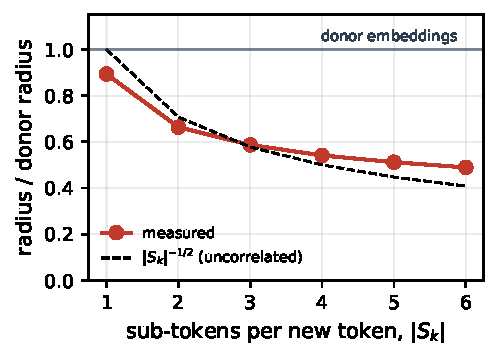
\includegraphics[width=\columnwidth]{figures/init_shrinkage.pdf}
\caption{Radius of the compositional estimate $\bm{c}_k$ relative to the donor
embedding radius, by the number of Qwen3 sub-tokens of the new token, for
20{,}000 candidate rows. Points are arithmetic mean centered radii; the
dashed line is the idealized root-mean-square reference
$|S_k|^{-1/2}$ from Proposition~\ref{prop:shrink}.}
\label{fig:init_shrinkage}
\end{figure}

Our \emph{analogical} estimate uses character-overlap similarity to tokens
of the old vocabulary. This is a lexical proxy, not an implementation of
the learned semantic auxiliary spaces of WECHSEL \cite{minixhofer2022wechsel}
or FOCUS \cite{dobler2023focus}. Donor tokens are converted to surface
strings by the base tokenizer. We strip surrounding whitespace and count
overlapping character 2--4-grams, using the whole stripped string as one
feature if it has no such gram. Let $P_g$ contain the first 400 donor IDs
having gram $g$, in ascending ID order, and let $q_k(g)$ be its target
count. Candidate $s$ receives score
$b_{ks}=\sum_g q_k(g)\mathbf{1}\{s\in P_g\}$.
The set $\mathcal{N}_k$ contains the ten highest positive scores, with
$w_s=b_{ks}/\sum_{j\in\mathcal{N}_k}b_{kj}$. Ties follow first encounter
when scanning grams by increasing length and position, then postings by ID.
With no candidate, we use the compositional estimate; if composition is
also unavailable, we use the random control defined below. With candidates
but no composition, the hybrid uses the analogical estimate alone. Then
\begin{equation}
\bm{a}_k = \sum_{s \in \mathcal{N}_k} w_s \bm{M}_s .
\label{eq:anal}
\end{equation}

The estimates use different surface information: the base tokenizer's
decomposition and character overlap with donor tokens. To test whether
combining them helps, LEP uses their average,
\begin{equation}
\bm{M}_{n+k} = \tfrac{1}{2}\left(\bm{c}_k + \bm{a}_k\right),
\label{eq:hybrid}
\end{equation}
and Proposition~\ref{prop:hybrid} gives its squared error relative to a
fixed reference row.

\begin{proposition}
\label{prop:hybrid}
Let $\bm{v}_k$ be the ideal row of $t_k$, and let $\bm{\varepsilon}_{\mathrm{c}} = \bm{c}_k - \bm{v}_k$ and
$\bm{\varepsilon}_{\mathrm{a}} = \bm{a}_k - \bm{v}_k$ be the errors of the two estimates. The error of
the hybrid~(\ref{eq:hybrid}) is
\begin{equation}
\lVert \bm{M}_{n+k} - \bm{v}_k \rVert^2
= \tfrac{1}{2}\left(\lVert\bm{\varepsilon}_{\mathrm{c}}\rVert^2 + \lVert\bm{\varepsilon}_{\mathrm{a}}\rVert^2\right)
- \tfrac{1}{4}\lVert \bm{c}_k - \bm{a}_k \rVert^2 .
\end{equation}
The hybrid error is therefore never larger than the mean of the two errors,
and it is smaller than the smaller of them whenever
$\lVert \bm{c}_k - \bm{a}_k \rVert^2 > 2\,\bigl|\lVert\bm{\varepsilon}_{\mathrm{c}}\rVert^2 - \lVert\bm{\varepsilon}_{\mathrm{a}}\rVert^2\bigr|$.
\end{proposition}

\emph{Proof.} Apply the parallelogram identity
$\lVert \bm{x} + \bm{y}\rVert^2 + \lVert \bm{x} - \bm{y}\rVert^2 = 2\lVert \bm{x}\rVert^2 + 2\lVert \bm{y}\rVert^2$
to $\bm{x} = \bm{\varepsilon}_{\mathrm{c}}$ and $\bm{y} = \bm{\varepsilon}_{\mathrm{a}}$, divide by four, and note that
$\bm{\varepsilon}_{\mathrm{c}} - \bm{\varepsilon}_{\mathrm{a}} = \bm{c}_k - \bm{a}_k$. \hfill$\square$

The identity bounds error against the mean component error; beating both
components requires the stronger condition stated above. Neither the ideal
row nor its component errors is observed, and Euclidean embedding error
does not by itself bound language-model loss. We therefore evaluate the
components and mixture empirically. The primary weight remains one half;
the mixture needs no data beyond the two component constructions.

\subsubsection{Gradient masking and selective unfreezing}

During adaptation, LEP keeps the original embedding rows fixed. A backward
hook sets their gradients to zero:
\begin{equation}
\nabla_{\bm{M}_i} \mathcal{L} =
\begin{cases}
0 & \text{if } i < n, \\
\nabla_{\bm{M}_i} \mathcal{L} & \text{otherwise.}
\end{cases}
\label{eq:mask}
\end{equation}
The masked embedding table is excluded from AdamW weight decay so that
zero-gradient rows remain fixed. Because the embeddings are tied, the hook also fixes the output rows of the
original vocabulary. LEP also adapts the top transformer layers to the new
segmentation: layers 24--27 of the 28-layer Qwen3 models. In the primary
0.6B policy, the 131{,}157 newly assigned vocabulary rows and four blocks
account for 197{,}228{,}544 effectively updated parameters; the rest stays
frozen. Fully trainable controls are specified below, and historical
layer-selection diagnostics appear in Appendix~\ref{app:layers}.

\section{Experimental Setup}
\label{sec:experiments}

The new adaptation study tests whether hybrid initialization changes Arabic language-modeling quality relative to its components and control initializers, and how the resulting recipe compares with continued pretraining (CPT) at the same nominal token budget. It also measures English likelihood and selected task accuracies after adaptation. These are separate endpoints; improved Arabic likelihood does not establish task transfer or English retention. Historical tokenizer and adaptation diagnostics are reported separately. Below we specify the data, models, training policies, metrics and statistical analysis.\footnote{AI assistance: OpenAI Codex~\cite{openaicodex2026}; see Acknowledgment.}

\subsection{Data}
\label{sec:data}

Tokenizer training and Arabic adaptation use the released \texttt{arb\_Arab} subset of FineWeb2-HQ \cite{fineweb2hq_2025}. The split manifest records a minimum document length of 200 characters and no additional positive quality-score cutoff. Corpus IDs are assigned deterministically to tokenizer-training, language-model-training, development and test buckets. The stored splits contain 159{,}826, 662{,}685, 2{,}522 and 6{,}602 documents, respectively. Development data monitor training; the final-step checkpoint is selected independently of development or test scores. Different IDs may still contain overlapping text. Appendix~\ref{app:protocol} gives the split and overlap-diagnostic details.

The new study reuses these previously inspected data and the released packed training streams; this follow-up therefore does not evaluate a new untouched holdout. English likelihood and downstream tasks use the separate datasets specified below.

\subsection{Models and baselines}

We use Qwen3-0.6B-Base and Qwen3-1.7B-Base \cite{qwen3technicalreport}, each with 28 transformer blocks and tied input and output embeddings; their hidden dimensions are 1{,}024 and 2{,}048. The released extended tokenizer is fixed before the new runs. Our primary LEP policy updates its newly assigned vocabulary rows and blocks 24--27 while preserving the original-token rows. CPT retains the base tokenizer and updates its embedding table and the same four blocks. Both policies freeze the final normalization parameters. Additional controls train every parameter of the extended model or base model, including the original embedding rows and final normalization. These fully trainable controls differ from the historical masked, all-layer LEP diagnostic.

For each setting, the initializer comparison includes random, constituent sub-token mean, moment-matched mean, character-$n$-gram analogical transfer and the equal-weight hybrid. The analogical component uses the implemented lexical proxy, not the pretrained auxiliary semantic embeddings of WECHSEL or FOCUS. At the smaller 0.6B budget, two additional mixtures give $\alpha\in\{0,.25,.5,.75,1\}$ together with the component endpoints. The primary $\alpha=.5$ is fixed; the sensitivity analysis does not select a replacement. Every registered arm uses training seeds 1, 2 and 3. Table~\ref{tab:design} gives the complete design.

The random control draws $\mathcal{N}(0,\sigma^2 I_d)$, where $I_d$ is the identity matrix for the backbone hidden dimension $d$ and $\sigma$ is the sample standard deviation across all entries of the original-token rows, excluding padding. The moment-matched control uses donor mean $\bm{\mu}$ and centered radii $r_i=\|\bm{M}_i-\bm{\mu}\|$. For $\bm{u}_k=\bm{c}_k-\bm{\mu}$ and a uniformly sampled donor row $J$, it assigns $\bm{\mu}+r_J\bm{u}_k/\|\bm{u}_k\|$ when $\|\bm{u}_k\|\geq10^{-6}$. Otherwise it draws $\bm{z}\sim\mathcal{N}(0,I_d)$ before sampling $J$ and assigns $\bm{\mu}+r_J\bm{z}/\sqrt d$. The regular branch matches sampled centered radii, not full covariance; the near-zero branch matches the expected squared radius. Empty base-tokenization results use the random fallback; the ordinary mean arm retains the library resize initialization. Initialization uses the recorded seed and float32 arithmetic before conversion to bfloat16 (BF16).

\begin{table}[t]
\centering\small
\fitcolumn{\begin{tabular}{lrrr}
\toprule
Setting & Steps & Arms & Runs \\
\midrule
0.6B, original budget & 2{,}000 & 10 & 30 \\
0.6B, nominal 500M & 5{,}087 & 8 & 24 \\
1.7B, original budget & 2{,}000 & 8 & 24 \\
\bottomrule
\end{tabular}}
\caption{The frozen 78-run adaptation design for LEP (ours) and CPT. Each setting contains five initializer arms, top-four-layer CPT and two fully trainable controls; the smaller 0.6B setting adds two mixture weights. Every arm has three training seeds. Tokenizer/model size, row policies and text exposure differ between LEP and CPT.}
\label{tab:design}
\end{table}

\subsection{Training}

The new runs use AdamW with learning rate $2\times10^{-4}$, linear decay, 10\% warmup and weight decay 0.01; embedding tables subject to frozen-row masking are excluded from decay. The global batch is nominally 96 packed sequences of 1{,}024 tokens. Runs last either 2{,}000 steps (196{,}608{,}000 nominal input tokens) or 5{,}087 steps (500{,}072{,}448 nominal input tokens). All settings use three training seeds. We evaluate the final completed step, with development-based checkpoint selection disabled. Actual input-token counts, successful-run wall time and peak allocated/reserved graphics processing unit (GPU) memory are recorded separately from nominal budgets; input tokens are not the number of unmasked prediction targets.

Equal nominal token budgets do not equalize consumed characters, model size, floating-point operations (FLOPs) or wall time. The packed streams use the respective tokenizers and have different lengths, so exposure and repetition can differ. Initialization and unsuccessful infrastructure attempts are accounted for separately. No run, seed or checkpoint is selected for favorable evaluation performance.

\subsection{Metrics}
\label{sec:metrics}

Intrinsic comparisons use Qwen as the unextended backbone control, DeepSeek-V3 as an additional multilingual BPE tokenizer and AraBERT \cite{antoun2020arabert} as an Arabic WordPiece baseline. The historical tokenizer evaluation reports fertility (tokens per whitespace-delimited word) and compression (Unicode characters per token) as per-document means, with corpus aggregates identified separately. The main intrinsic artifact uses 5{,}000 test documents; the 80K algorithm/preprocessing comparison uses 2{,}000. The baseline table gives raw and common-normalized inputs, and its figure uses common-normalized inputs. Algorithm and pruning comparisons use each tokenizer's saved normalization. Word-level out-of-vocabulary (OOV) rates and unknown-token (UNK) fractions accompany compression comparisons, since an unknown token can conceal unsupported input; unscored rates are marked separately. Tokens per morpheme is a corpus ratio over the first 500 test documents: total tokenizer tokens divided by total CAMeL \texttt{d3tok} segments \cite{obeid2020camel}. CAMeL receives common normalized text, while each tokenizer receives its declared own-normalized input. These diagnostics do not constitute additional training seeds in the new study.

Language-model evaluation uses a common-text protocol. For each document, the alif-preserving paper normalizer is applied to a fixed point before taking at most 512 Unicode code points. The normalizer includes Latin lowercasing, so the English endpoint is normalized-text likelihood. The same canonical span is scored by every compared model, without tokenizer-specific truncation. An explicit common conditioning token (ID 151643) precedes the target; every target token contributes to the summed negative log likelihood, while the conditioning token is excluded. Let $c$ be the canonical character span, $(t_1,\ldots,t_m)$ its target-token sequence and $t_0$ the common conditioning token. Negative log likelihood (NLL) in nats is $\mathrm{NLL}(t_i)=-\ln p(t_i\mid t_0,\ldots,t_{i-1})$. We compute
\begin{equation}
\mathrm{BPC}(c)=\frac{\sum_i\mathrm{NLL}(t_i)}{|c|\ln 2}.
\label{eq:bpc}
\end{equation}
The primary aggregate is the mean of document BPC values; corpus BPC divides total negative log likelihood by the total character count. The Arabic cohort is the first 1{,}500 eligible documents in the stored test order, and the English cohort is the first 1{,}000 WikiText-103 \cite{merity2017pointer} raw test rows of at least 200 raw characters. Source hashes, canonical hashes, character counts and evaluation protocols must match across comparisons. Historical values obtained from independently truncated 1{,}024-token spans remain separate and are not used as common-text comparisons.

The fixed downstream panel evaluates seven logical checkpoints: one pinned 0.6B base and all three training seeds of the nominal-500M hybrid and top-four-layer CPT arms. Five Arabic tasks from the Open Arabic LLM Leaderboard (OALL) v2 \cite{OALL-2} (ArabicMMLU \cite{koto2024arabicmmlu}, MadinahQA, Arabic EXAMS \cite{hardalov2020exams}, AraTrust \cite{alghamdi2024aratrust} and AlGhafa \cite{almazrouei2023alghafa}) and two English tasks (MMLU \cite{hendrycks2021measuring} and ARC-Easy \cite{clark2018arc}) give 49 checkpoint--task blocks. The Arabic endpoint is unweighted mean accuracy across the five fixed tasks; pooled accuracy and every task score are also reported. The English task endpoint is the unweighted mean of its two tasks. These are custom-protocol subset measurements, not official leaderboard submissions. Task accuracy at 1.7B or under the fully trainable controls is outside this panel.

We report measured training time and peak memory separately from tokenizer compression, and use a fixed serving workload to measure tokenization, prefill, decode, generation and end-to-end timing, generated-token/character throughput and peak memory at their recorded measurement scopes.

\subsection{Statistical analysis}

For the new study, individual training-seed outcomes and their mean and sample standard deviation are retained. Arabic BPC inference uses a crossed paired bootstrap \cite{efron1979bootstrap} over the three training seeds and common documents, with 10{,}000 replicates and resampling seed 42. We report marginal 95\% percentile intervals and two-sided, centered-bootstrap Monte Carlo $p$-values with the plus-one correction. Holm correction \cite{holm1979simple} is applied separately to the six predefined LEP--CPT contrasts (two parameter policies at each of three settings) and the twelve hybrid--initializer contrasts (four controls at each setting). An incomplete family receives no inferential conclusion. The original-budget mixture-weight sensitivity is exploratory and does not select the primary initializer.

The downstream family contains nine contrasts: hybrid--CPT, hybrid--base and CPT--base for Arabic macro task accuracy, English macro task accuracy and English macro document BPC. The task bootstrap draws training seeds jointly across the fixed tasks and resamples paired items within each task; tasks themselves are not resampled. The fixed base is repeated as a reference, not treated as three independently trained models. Inference and Holm-adjusted $p$-values are withheld until the complete nine-contrast family validates. All per-task and per-seed values remain visible. No equivalence or noninferiority margin is defined, so nonsignificance does not establish preserved performance.

\section{Results}
\label{sec:results}

We first examine tokenization and pruning, then controlled adaptation and
initialization, followed by resource use and Arabic task accuracy with
English retention.\footnote{AI assistance: OpenAI Codex~\cite{openaicodex2026}; see Acknowledgment.}

\subsection{AraToken against existing tokenizers}
\label{sec:res_tokenizers}

Table~\ref{tab:baseline_comparison} and Figure~\ref{fig:baseline_comparison}
compare our AraToken with the tokenizers of Qwen2.5/Qwen3, DeepSeek-V3 and
AraBERT. AraToken gives the lowest fertility and the highest compression of
all systems. On normalized text it needs 1.212 tokens per word, against 2.179
for Qwen2.5/Qwen3, 2.177 for DeepSeek-V3 and 1.833 for AraBERT. This is
44.4\% fewer tokens than the tokenizer of Qwen3 and 33.9\% fewer than AraBERT,
and each token covers 4.80 characters, against 2.67 and 3.17. AraToken also
leads on raw, unnormalized text, where it needs 40.1\% fewer tokens than the
tokenizer of Qwen3. Raw-input results still include each tokenizer's
internal preprocessing and do not isolate segmentation alone.

% generated by scripts/experiments/make_tables.py -- do not edit
\begin{table}[!ht]
\centering
\small
\setlength{\tabcolsep}{4pt}
\fitcolumn{\begin{tabular}{@{}lrrrr@{}}
\toprule
\textbf{Tokenizer} & \textbf{Vocab} & \multicolumn{2}{c}{\textbf{Fertility} $\downarrow$} & \textbf{Compr.} $\uparrow$ \\
 & & raw & norm. & norm. \\
\midrule
Qwen2.5 & 151{,}665 & 2.283 & 2.179 & 2.669 \\
DeepSeek-V3 & 128{,}815 & 2.238 & 2.177 & 2.670 \\
AraBERT & 64{,}000 & 1.796 & 1.833 & 3.170 \\
\midrule
\multicolumn{5}{@{}l}{\textit{Ours, pruned}} \\
AraToken, 95\% coverage & 60{,}149 & 1.431 & 1.281 & 4.549 \\
AraToken, 99\% coverage & 109{,}844 & 1.380 & 1.227 & 4.745 \\
\midrule
\multicolumn{5}{@{}l}{\textit{Ours, full scale}} \\
\textbf{AraToken, 150K} & 150{,}000 & \textbf{1.366} & \textbf{1.212} & \textbf{4.802} \\
AraToken, 150K, byte fallback & 150{,}000 & 1.512 & 1.215 & 4.792 \\
\bottomrule
\end{tabular}}
\caption{AraToken against existing tokenizers on 5{,}000 \texttt{test} documents. Fertility is tokens per word and compression is characters per token, both as per-document means. Every tokenizer is measured on raw text and on common text normalized by the AraToken pipeline. Qwen3 has 151{,}669 token IDs and the same displayed scores as Qwen2.5. The best values are in bold.}
\label{tab:baseline_comparison}
\end{table}


\begin{figure*}[t]
\centering
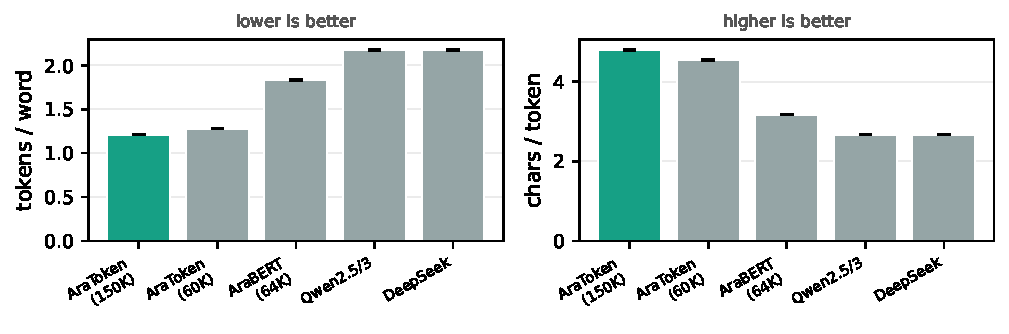
\includegraphics[width=\textwidth]{figures/baseline_comparison.pdf}
\caption{Fertility (left, lower is better) and compression (right, higher is
better) of AraToken (ours) and existing tokenizers on 5{,}000 test documents with
common externally normalized input and 95\% bootstrap intervals.}
\label{fig:baseline_comparison}
\end{figure*}

Part of the gap to AraBERT could come from vocabulary size, since AraToken has
150K pieces and AraBERT 64K. Our pruned AraToken with 95\% coverage has
60{,}149 pieces, fewer than AraBERT, and it still needs 30.1\% fewer tokens
per word. The advantage therefore persists at a similar vocabulary size. This
comparison does not isolate vocabulary size from segmentation, training data
or normalization. AraToken also needs the fewest
tokens per morpheme: 0.89, against 1.32 for AraBERT and 1.57 for Qwen3, with
morphemes from the CAMeL Tools analyzer. This corpus ratio describes granularity relative to the analyzer's
reference; it is not a measure of morpheme-boundary accuracy. On dialectal tweets from ArSarcasm,
a register far from its training corpus, our AraToken byte-fallback variant still
needs 21.8\% fewer tokens per word than the tokenizer of Qwen3
(Appendix~\ref{app:dialect}).

\subsection{Choice of segmentation algorithm}
\label{sec:res_algorithms}

Table~\ref{tab:tokenizer_results} compares BPE, WordPiece and Unigram, trained
on the same corpus at an 80K vocabulary, with and without the steps of the
normalization pipeline. Unigram gives the lowest fertility and the highest
compression in every configuration. Our full-pipeline Unigram configuration needs 1.245
tokens per word, against 1.295 for BPE and 1.296 for WordPiece, and it covers
4.69 characters per token, against 4.51 for both. Its rate of unknown words is
0.28\% in this 80K comparison. A separate 150K byte-fallback variant is
evaluated in Appendix~\ref{app:dialect}.

% generated by scripts/experiments/make_tables.py -- do not edit
\begin{table}[t]
\centering
\small
\fitcolumn{\begin{tabular}{lccc}
\toprule
\textbf{Tokenizer} & \textbf{Fertility} & \textbf{Compression} & \textbf{OOV\%} \\
\midrule
\multicolumn{4}{l}{\textit{Diacritics removed}} \\
BPE & 1.303 & 4.49 & -- \\
BPE + char.\ rules & 1.295 & 4.51 & -- \\
Unigram & 1.253 & 4.66 & 0.14 \\
\textbf{Unigram + char.\ rules} & 1.245 & 4.69 & 0.28 \\
WordPiece & 1.304 & 4.48 & 0.00 \\
WordPiece + char.\ rules & 1.296 & 4.51 & 0.00 \\
\midrule
\multicolumn{4}{l}{\textit{Diacritics kept}} \\
BPE & 1.400 & 4.33 & -- \\
BPE + char.\ rules & 1.392 & 4.35 & -- \\
Unigram & 1.286 & 4.62 & 0.15 \\
Unigram + char.\ rules & 1.278 & 4.64 & 0.28 \\
WordPiece & 1.402 & 4.32 & 0.00 \\
WordPiece + char.\ rules & 1.395 & 4.34 & 0.00 \\
\bottomrule
\end{tabular}}
\caption{Segmentation algorithms at an 80K vocabulary, trained on \texttt{tok-train} and measured on 2{,}000 \texttt{test} documents under each tokenizer's own normalization. ``Char.\ rules'' adds the character rules of Table~\ref{tab:normalization}. Unigram with the full pipeline (bold) gives the lowest fertility and the highest compression. OOV is scored on the first 500 documents, with 224{,}412--224{,}503 words depending on normalization. ``--'' means not scored (BPE has no usable UNK marker).}
\label{tab:tokenizer_results}
\end{table}


Both steps of our normalization pipeline lower fertility for all three algorithms
(Figure~\ref{fig:fertility}). Removing diacritics gives the larger gain: 7.0\%
for BPE, 7.1\% for WordPiece and 2.6\% for Unigram. The character rules add
about 0.6\% for each algorithm, and the full pipeline lowers fertility by
7.5\%, 7.6\% and 3.2\%.

\begin{figure}[t]
\centering
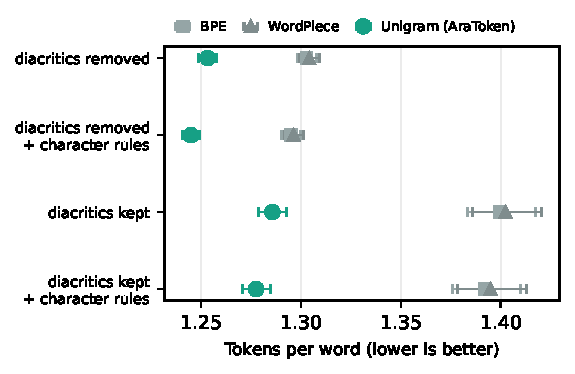
\includegraphics[width=\columnwidth]{figures/fertility_comparison.pdf}
\caption{Fertility under AraToken normalization ablations (ours), evaluated with three segmentation algorithms on the \texttt{test}
split under four preprocessing configurations: 2{,}000 documents with each
tokenizer's saved normalization and 95\% bootstrap intervals.}
\label{fig:fertility}
\end{figure}

\subsection{Vocabulary pruning}
\label{sec:res_pruning}

Table~\ref{tab:pruning_results} and Figure~\ref{fig:pruning} show the cost of
pruning. At 99\% coverage the vocabulary shrinks by 27\%, to 109{,}844
pieces, and fertility rises by 1.2\%, from 1.212 to 1.227. At 95\% coverage it
shrinks by 60\%, to 60{,}149 pieces, for a rise of 5.7\% to 1.281. Both of our pruned
tokenizers stay well ahead of every baseline in
Table~\ref{tab:baseline_comparison}. Pruning removes the long and rare pieces
of the vocabulary (Appendix~\ref{app:pruning}), so one coverage threshold sets the trade-off
between vocabulary size and fertility.

% generated by scripts/experiments/make_tables.py -- do not edit
\begin{table}[t]
\centering
\small
\fitcolumn{\fitcolumn{\begin{tabular}{@{}lrrr@{}}
\toprule
\textbf{Configuration} & \textbf{Vocab} & \textbf{Fertility} $\downarrow$ & \textbf{Compr.} $\uparrow$ \\
\midrule
full vocabulary & 150{,}000 & 1.212 & 4.80 \\
99\% coverage & 109{,}844 & 1.227 & 4.74 \\
95\% coverage & 60{,}149 & 1.281 & 4.55 \\
\bottomrule
\end{tabular}}}
\caption{AraToken (ours) pruned by corpus coverage, measured on the first 5{,}000 \texttt{test} documents under each tokenizer's own normalization.}
\label{tab:pruning_results}
\end{table}


\begin{figure}[t]
\centering
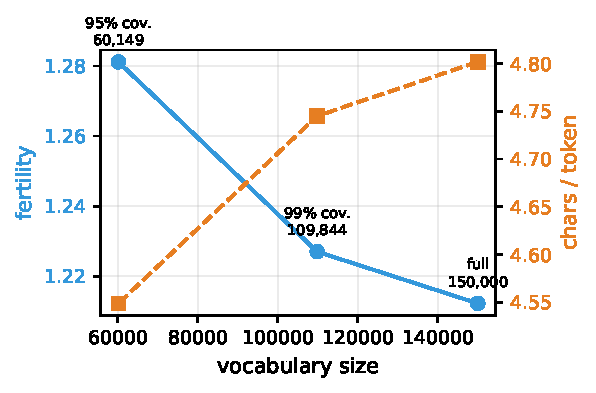
\includegraphics[width=\columnwidth]{figures/vocab_pruning.pdf}
\caption{Vocabulary size and fertility of AraToken (ours) at full size and at 99\%
and 95\% coverage.}
\label{fig:pruning}
\end{figure}

\subsection{Adaptation quality}
\label{sec:res_lep}

Tables~\ref{tab:rebuttal-fair-estimates} and
\ref{tab:rebuttal-fair-inference} report all six controlled LEP--CPT
comparisons. Every arm contains three completed training seeds evaluated
on the same 1{,}500 canonical Arabic spans. LEP uses the fixed half-weight
initializer. Top-four-layer comparisons allow embedding adaptation in
both methods; the additional fully trainable pairs update every parameter.
The comparison is at matched nominal packed-token budgets, not equal
compute or equal character exposure.

With the top-four policy, our LEP reaches 1.4111 versus 1.5138 BPC at 2{,}000
steps, 1.3551 versus 1.4782 at the nominal-500M budget, and 1.3224 versus
1.3577 at 1.7B. The paired LEP--CPT differences are $-0.1027$, $-0.1231$
and $-0.0353$ BPC; their marginal 95\% intervals are
$[-0.1066,-0.0989]$, $[-0.1277,-0.1187]$ and $[-0.0395,-0.0313]$.
The fully trainable controls retain advantages of 0.0986, 0.1029 and
0.0611 BPC in the same order. All six differences survive the declared
Holm correction ($p_{\mathrm{Holm}}=0.000600$).

These controls support a canonical-Arabic likelihood benefit under both
trainability policies and at both base-model sizes. They do not isolate
segmentation from normalization, character exposure or the additional
embedding capacity. The resource comparison below records the higher
training cost, and the task and English measurements test separate
outcomes. Individual seeds and all declared initializer arms are retained
in the accompanying result files.

\begin{table*}[t]
\centering
\small
\setlength{\tabcolsep}{4pt}
\begin{tabular}{@{}lllllll@{}}
\toprule
Model & Steps & Trainability & CPT Arabic $\downarrow$ & LEP Arabic $\downarrow$ & CPT English $\downarrow$ & LEP English $\downarrow$ \\
\midrule
0.6B & 2,000 & Top four & 1.5138 $\pm$ 0.0005 & 1.4111 $\pm$ 0.0003 & 1.2249 $\pm$ 0.0014 & 1.2080 $\pm$ 0.0006 \\
0.6B & 2,000 & Full & 1.3780 $\pm$ 0.0009 & 1.2794 $\pm$ 0.0039 & 1.3407 $\pm$ 0.0103 & 1.2945 $\pm$ 0.0070 \\
0.6B & 5,087 & Top four & 1.4782 $\pm$ 0.0004 & 1.3551 $\pm$ 0.0017 & 1.2430 $\pm$ 0.0014 & 1.2159 $\pm$ 0.0008 \\
0.6B & 5,087 & Full & 1.3226 $\pm$ 0.0022 & 1.2197 $\pm$ 0.0006 & 1.3669 $\pm$ 0.0030 & 1.3090 $\pm$ 0.0025 \\
1.7B & 2,000 & Top four & 1.3577 $\pm$ 0.0010 & 1.3224 $\pm$ 0.0029 & 1.0842 $\pm$ 0.0033 & 1.0721 $\pm$ 0.0011 \\
1.7B & 2,000 & Full & 1.2699 $\pm$ 0.0009 & 1.2088 $\pm$ 0.0010 & 1.1207 $\pm$ 0.0024 & 1.1183 $\pm$ 0.0039 \\
\bottomrule
\end{tabular}
\caption{Arabic macro document BPC on 1,500 shared canonical documents, each truncated to at most 512 Unicode characters. Lower BPC is better. Values are means $\pm$ sample standard deviation (SD) across three paired training seeds. English uses 1,000 canonical documents with the same prefix rule and is descriptive. Top-four LEP updates new embedding rows and the last four transformer layers; CPT updates all original embedding rows and the same layers. Full pairs update all parameters. LEP (ours) uses the predeclared half mixture. Matched nominal packed-token budgets do not imply equal compute or text exposure. The held-out data had previously been inspected. }
\label{tab:rebuttal-fair-estimates}
\end{table*}

\begin{table*}[t]
\centering
\small
\setlength{\tabcolsep}{4pt}
\begin{tabular}{@{}llllll@{}}
\toprule
Model & Steps & Trainability & $\Delta$ BPC $\downarrow$ & 95\% interval & Holm $p$ \\
\midrule
0.6B & 2,000 & Top four & -0.1027 & [-0.1066, -0.0989] & 0.00059994 \\
0.6B & 2,000 & Full & -0.0986 & [-0.1033, -0.0937] & 0.00059994 \\
0.6B & 5,087 & Top four & -0.1231 & [-0.1277, -0.1187] & 0.00059994 \\
0.6B & 5,087 & Full & -0.1029 & [-0.1077, -0.0987] & 0.00059994 \\
1.7B & 2,000 & Top four & -0.0353 & [-0.0395, -0.0313] & 0.00059994 \\
1.7B & 2,000 & Full & -0.0611 & [-0.0646, -0.0577] & 0.00059994 \\
\bottomrule
\end{tabular}
\caption{Arabic macro document BPC on 1,500 shared canonical documents, each truncated to at most 512 Unicode characters. Lower BPC is better. LEP (ours) minus CPT for all six trainability comparisons. Negative differences favor LEP. Intervals are 95\% marginal crossed seed/document bootstrap intervals over three paired training seeds and 1,500 shared documents; they are not simultaneous intervals. Holm correction covers the six planned fairness contrasts. The held-out data had previously been inspected. }
\label{tab:rebuttal-fair-inference}
\end{table*}


\subsection{Initialization of the new rows}
\label{sec:res_init}

Tables~\ref{tab:rebuttal-initializer-ar} and
\ref{tab:rebuttal-initializer-inference} compare our fixed half-weight mixture with compositional mean,
moment-matched mean, character-ngram analogical transfer and random
initialization under all three scale/budget settings. These comparisons
hold the extended tokenizer, trainable policy and schedule fixed within
each setting. The character-ngram method is a lexical proxy, not a
reimplementation of WECHSEL or FOCUS.

Against compositional initialization, our mixture lowers Arabic BPC by
0.0485 at the original 0.6B budget, 0.0402 at the nominal-500M budget and
0.0439 at 1.7B. Its advantages over analogical initialization are smaller:
0.0063 at the original budget and 0.0117 at 1.7B, with marginal 95\%
intervals for mixture minus analogical of $[-0.0080,-0.0043]$ and
$[-0.0135,-0.0097]$. These comparisons survive Holm correction over the
12 declared initializer contrasts ($p_{\mathrm{Holm}}=0.0012$).
At the nominal-500M budget, the difference from analogical initialization
is unresolved: $-0.0009$ BPC, interval $[-0.0028,0.0010]$,
$p_{\mathrm{Holm}}=0.383$; one of the three seed differences favors the
analogical component. Random and moment-matched initialization have
higher Arabic BPC in all three settings.

The mixture therefore improves on both components in two of the three
settings, while its advantage over the stronger component narrows at the
larger 0.6B budget. This is a budget-dependent empirical result, not a
consequence of the squared-error identity or evidence that either
component fails in isolation. With only three training seeds, the
crossed-bootstrap intervals have limited coverage of training variability.

In the exploratory original-budget sweep, where $\alpha$ is the
compositional weight, Arabic BPC is 1.4174, 1.4052, 1.4111, 1.4289 and
1.4596 at $\alpha=0,0.25,0.5,0.75,1$, respectively. The observed minimum
is at 0.25. We retain the predeclared half-weight mixture as the primary
method; these results do not establish that equal weighting is optimal.
Table~\ref{tab:rebuttal-initializer-en} reports English likelihood for every
initializer; Table~\ref{tab:rebuttal-alpha} gives the complete sensitivity
sweep. The endpoint at $\alpha=1$ is represented by the declared
compositional-only arm, not an additional trained mixture. All individual
seed values are retained.

\begin{table*}[t]
\centering
\small
\setlength{\tabcolsep}{4pt}
\begin{tabular}{@{}llll@{}}
\toprule
Initializer & \shortstack{0.6B / 2,000 steps\\BPC $\downarrow$} & \shortstack{0.6B / 5,087 steps\\BPC $\downarrow$} & \shortstack{1.7B / 2,000 steps\\BPC $\downarrow$} \\
\midrule
Compositional mean & 1.4596 $\pm$ 0.0018 & 1.3953 $\pm$ 0.0007 & 1.3664 $\pm$ 0.0042 \\
Moment-matched mean & 1.5362 $\pm$ 0.0058 & 1.4534 $\pm$ 0.0043 & 1.4698 $\pm$ 0.0085 \\
Character-ngram analogical proxy & 1.4174 $\pm$ 0.0014 & 1.3560 $\pm$ 0.0012 & 1.3341 $\pm$ 0.0025 \\
Half mixture (ours) & 1.4111 $\pm$ 0.0003 & 1.3551 $\pm$ 0.0017 & 1.3224 $\pm$ 0.0029 \\
Random & 2.3270 $\pm$ 0.0082 & 2.0906 $\pm$ 0.0118 & 2.1965 $\pm$ 0.0131 \\
\bottomrule
\end{tabular}
\caption{Arabic macro document BPC on 1,500 shared canonical documents, each truncated to at most 512 Unicode characters. Lower BPC is better. Values are means $\pm$ sample standard deviation (SD) across three paired training seeds. All five predeclared initializers use the top-four training policy. The analogical initializer is a character-ngram proxy. No initializer is selected from these results. The held-out data had previously been inspected. }
\label{tab:rebuttal-initializer-ar}
\end{table*}

\begin{table*}[t]
\centering
\small
\setlength{\tabcolsep}{4pt}
\begin{tabular}{@{}llll@{}}
\toprule
Initializer & \shortstack{0.6B / 2,000 steps\\BPC $\downarrow$} & \shortstack{0.6B / 5,087 steps\\BPC $\downarrow$} & \shortstack{1.7B / 2,000 steps\\BPC $\downarrow$} \\
\midrule
Compositional mean & 1.2087 $\pm$ 0.0008 & 1.2172 $\pm$ 0.0009 & 1.0705 $\pm$ 0.0008 \\
Moment-matched mean & 1.2111 $\pm$ 0.0005 & 1.2212 $\pm$ 0.0008 & 1.0740 $\pm$ 0.0019 \\
Character-ngram analogical proxy & 1.2069 $\pm$ 0.0007 & 1.2136 $\pm$ 0.0015 & 1.0722 $\pm$ 0.0014 \\
Half mixture (ours) & 1.2080 $\pm$ 0.0006 & 1.2159 $\pm$ 0.0008 & 1.0721 $\pm$ 0.0011 \\
Random & 1.2252 $\pm$ 0.0019 & 1.2450 $\pm$ 0.0015 & 1.0807 $\pm$ 0.0017 \\
\bottomrule
\end{tabular}
\caption{English macro document BPC on 1,000 shared canonical documents, each truncated to at most 512 Unicode characters. Lower BPC is better. English results are descriptive only. Values are means $\pm$ sample standard deviation (SD) across three paired training seeds. All five predeclared initializers use the top-four training policy. The analogical initializer is a character-ngram proxy. No initializer is selected from these results. The held-out data had previously been inspected. }
\label{tab:rebuttal-initializer-en}
\end{table*}

\begin{table*}[t]
\centering
\small
\setlength{\tabcolsep}{4pt}
\begin{tabular}{@{}llllll@{}}
\toprule
Model & Steps & Comparator & $\Delta$ BPC $\downarrow$ & 95\% interval & Holm $p$ \\
\midrule
0.6B & 2,000 & Compositional mean & -0.0485 & [-0.0509, -0.0463] & 0.00119988 \\
0.6B & 2,000 & Moment-matched mean & -0.1251 & [-0.1305, -0.1192] & 0.00119988 \\
0.6B & 2,000 & Character-ngram analogical proxy & -0.0063 & [-0.0080, -0.0043] & 0.00119988 \\
0.6B & 2,000 & Random & -0.9159 & [-0.9278, -0.9041] & 0.00119988 \\
0.6B & 5,087 & Compositional mean & -0.0402 & [-0.0420, -0.0384] & 0.00119988 \\
0.6B & 5,087 & Moment-matched mean & -0.0984 & [-0.1036, -0.0923] & 0.00119988 \\
0.6B & 5,087 & Character-ngram analogical proxy & -0.0009 & [-0.0028, +0.0010] & 0.382562 \\
0.6B & 5,087 & Random & -0.7355 & [-0.7484, -0.7221] & 0.00119988 \\
1.7B & 2,000 & Compositional mean & -0.0439 & [-0.0460, -0.0418] & 0.00119988 \\
1.7B & 2,000 & Moment-matched mean & -0.1474 & [-0.1578, -0.1365] & 0.00119988 \\
1.7B & 2,000 & Character-ngram analogical proxy & -0.0117 & [-0.0135, -0.0097] & 0.00119988 \\
1.7B & 2,000 & Random & -0.8741 & [-0.8873, -0.8609] & 0.00119988 \\
\bottomrule
\end{tabular}
\caption{Arabic macro document BPC on 1,500 shared canonical documents, each truncated to at most 512 Unicode characters. Lower BPC is better. Half-mixture LEP (ours) minus each initializer comparator, with the top-four training policy. Negative differences favor the half mixture. Intervals are 95\% marginal crossed seed/document bootstrap intervals over three paired training seeds and 1,500 shared documents; they are not simultaneous intervals. Holm correction covers all 12 planned initializer contrasts. The held-out data had previously been inspected. }
\label{tab:rebuttal-initializer-inference}
\end{table*}

\begin{table*}[t]
\centering
\small
\setlength{\tabcolsep}{4pt}
\begin{tabular}{@{}llll@{}}
\toprule
$\alpha$ & Initializer & Arabic BPC $\downarrow$ & English BPC $\downarrow$ \\
\midrule
0.00 & Character-ngram analogical proxy & 1.4174 $\pm$ 0.0014 & 1.2069 $\pm$ 0.0007 \\
0.25 & Quarter compositional & 1.4052 $\pm$ 0.0007 & 1.2090 $\pm$ 0.0007 \\
0.50 & Half mixture (ours) & 1.4111 $\pm$ 0.0003 & 1.2080 $\pm$ 0.0006 \\
0.75 & Three-quarters compositional & 1.4289 $\pm$ 0.0006 & 1.2069 $\pm$ 0.0004 \\
1.00 & Compositional mean & 1.4596 $\pm$ 0.0018 & 1.2087 $\pm$ 0.0008 \\
\bottomrule
\end{tabular}
\caption{Arabic macro document BPC on 1,500 shared canonical documents, each truncated to at most 512 Unicode characters. Lower BPC is better. Values are means $\pm$ sample standard deviation (SD) across three paired training seeds. Complete exploratory five-point mixture sweep at 0.6B, 2,000 steps, top-four training. $\alpha$ weights the compositional component; $1-\alpha$ weights the character-ngram analogical proxy. Endpoints reuse the component runs. The predeclared primary value remains $\alpha=0.5$. English uses 1,000 canonical documents with the same prefix rule and is descriptive. The held-out data had previously been inspected. }
\label{tab:rebuttal-alpha}
\end{table*}


\subsection{Compression, training cost and serving}
\label{sec:res_eff}

The released packed adaptation streams contain 448{,}343{,}040 input
tokens with the extended tokenizer and 802{,}561{,}024 with the base
tokenizer. Fewer tokens therefore represent the same source corpus,
subject to the packing remainders described in Appendix~\ref{app:hparams}.
This is an input-compression result, not a generation-throughput measurement.
At 2{,}000 steps both methods consume 196{,}608{,}000 packed input tokens;
their character exposure and FLOPs differ. At 5{,}087 steps, actual counts
are 500{,}097{,}024 for our LEP and 500{,}072{,}448 for CPT because of a partial
accumulation group at the extended stream's epoch boundary.

Measured training cost is higher for our LEP. For the top-four-layer pairs,
mean trainer runtime is 1.25 times CPT at each 0.6B budget and 1.28 times
CPT at 1.7B; peak allocated memory ratios are 1.77, 1.77 and 1.67,
respectively. Fully trainable LEP takes 1.23, 1.23 and 1.25 times the
corresponding CPT runtime. These are measured runtime ratios on the
recorded H100 workers, not controlled estimates of FLOPs.
Across all 78 successful training runs, summed trainer runtime is
272.57 single-GPU hours. Initialization, evaluation and infrastructure
failures are accounted for separately; incomplete timing records for the
quarantined launch prevent an exact total campaign-cost claim.
Table~\ref{tab:rebuttal-training-resources} gives absolute training costs.

Table~\ref{tab:rebuttal-serving} reports all six fixed-checkpoint serving
measurements. At 0.6B, our LEP and CPT have similar observed token rates:
61.61 versus 61.53 tokens/s at batch one and 227.09 versus 228.35 at
batch four. At 1.7B, LEP is slower: 55.67 versus 56.95 and 206.99 versus
208.78 tokens/s. Generated-character throughput is 1.51--1.65 times CPT
across these settings, while allocated memory is higher. The generated
strings differ and can become repetitive, so the character-rate gain
is not a quality-adjusted speedup or a reduction in equal-output latency.
The table and raw records separate end-to-end batch time, generation
throughput and memory; no serving significance claim is made.

\begin{table*}[t]
\centering
\small
\setlength{\tabcolsep}{4pt}
\begin{tabular}{@{}lllllll@{}}
\toprule
Model & Steps & Trainability & CPT hours $\downarrow$ & LEP hours $\downarrow$ & \shortstack{CPT peak\\allocated GiB $\downarrow$} & \shortstack{LEP peak\\allocated GiB $\downarrow$} \\
\midrule
0.6B & 2,000 & Top four & 1.793 & 2.236 & 16.792 & 29.773 \\
0.6B & 2,000 & Full & 1.932 & 2.370 & 18.916 & 31.898 \\
0.6B & 5,087 & Top four & 4.530 & 5.654 & 16.792 & 29.773 \\
0.6B & 5,087 & Full & 4.881 & 6.013 & 18.916 & 31.898 \\
1.7B & 2,000 & Top four & 2.557 & 3.281 & 21.013 & 34.993 \\
1.7B & 2,000 & Full & 2.855 & 3.566 & 27.795 & 41.775 \\
\bottomrule
\end{tabular}
\caption{Successful training resources on H100 80GB GPUs for the six predeclared CPT/half-mixture LEP (ours) comparisons. Hours are mean train\_runtime per run over three training seeds, including in-loop validation/checkpoint work; initialization, model/data preparation, final-model save and separate evaluations are excluded. Device allocated memory is the maximum across the three runs, including resident model memory. These values are not total campaign cost: initialization and failed attempts are accounted separately, with missing timing endpoints for quarantined attempts. Matched nominal packed-token budgets do not imply equal actual tokens, text exposure or compute. Full pairs update every parameter; top-four policies differ in embedding-row updates.}
\label{tab:rebuttal-training-resources}
\end{table*}

\begin{table*}[t]
\centering
\small
\setlength{\tabcolsep}{4pt}
\begin{tabular}{@{}lllllll@{}}
\toprule
Model & Batch & \shortstack{Mean end-to-end\\s/batch $\downarrow$} & \shortstack{Generation\\tokens/s $\uparrow$} & \shortstack{Generated\\characters/s $\uparrow$} & \shortstack{Peak allocated\\GiB $\downarrow$} & \shortstack{Peak reserved\\GiB $\downarrow$} \\
\midrule
0.6B Base & 1 & 2.082 & 61.51 & 145.56 & 1.170 & 1.195 \\
0.6B Base & 4 & 2.243 & 228.46 & 543.60 & 1.259 & 1.344 \\
0.6B CPT & 1 & 2.082 & 61.53 & 147.67 & 1.170 & 1.195 \\
0.6B CPT & 4 & 2.244 & 228.35 & 555.14 & 1.259 & 1.348 \\
0.6B LEP & 1 & 2.079 & 61.61 & 243.61 & 1.415 & 1.439 \\
0.6B LEP & 4 & 2.256 & 227.09 & 864.41 & 1.489 & 1.582 \\
1.7B Base & 1 & 2.127 & 60.21 & 147.55 & 3.265 & 3.279 \\
1.7B Base & 4 & 2.271 & 225.67 & 564.12 & 3.353 & 3.445 \\
1.7B CPT & 1 & 2.249 & 56.95 & 138.58 & 3.265 & 3.279 \\
1.7B CPT & 4 & 2.454 & 208.78 & 504.77 & 3.353 & 3.445 \\
1.7B LEP & 1 & 2.300 & 55.67 & 212.71 & 3.759 & 3.771 \\
1.7B LEP & 4 & 2.475 & 206.99 & 763.33 & 3.832 & 3.912 \\
\bottomrule
\end{tabular}
\caption{Descriptive serving measurements including LEP (ours) on one H100 80GB GPU, in the displayed model order. All models use the same 32 canonical Arabic prompts of 256 Unicode characters, 128 greedy new tokens, batches 1 and 4, two warmup batches per batch size, brain floating-point 16 (BF16), left padding and key--value (KV) caching, without end-of-sequence (EOS) stopping. Bases are fixed checkpoints rerun in this sequence; adapted checkpoints use predeclared training seed 1 (0.6B: 5,087 steps; 1.7B: 2,000 steps; top-four policy). Mean end-to-end seconds per batch equals total end-to-end time divided by 32 or 8 measured batches, respectively; it is not per-request latency. End-to-end includes tokenization, host/device transfers, generation and text decoding, excluding model loading. Throughput uses 4,096 generated tokens or the observed decoded Unicode-character count, respectively, divided by total generation time. Memory is maximum device allocated/reserved memory across batches, including the model. Generated content differs and can repeat after EOS; character throughput is content-dependent and is not quality-adjusted utility or equal-output latency. Full phase timings and generated content are retained in the raw records. No serving significance claim is made.}
\label{tab:rebuttal-serving}
\end{table*}


\subsection{Arabic task accuracy and English retention}
\label{sec:res_tasks}

Table~\ref{tab:rebuttal-downstream-estimates} includes all 49 task blocks
for the fixed base and three seeds each of nominal-500M top-four LEP and
CPT. Our LEP achieves the highest Arabic macro point estimate: 40.65\%,
compared with 39.58\% for CPT and 39.20\% for the base. Its mean accuracy
exceeds CPT on MadinahQA (41.28\% versus 38.31\%), ArabicEXAMS
(30.91\% versus 29.73\%) and AlGhafa (44.87\% versus 39.44\%).
LEP also exceeds the base on these three tasks and AraTrust.
The LEP--CPT macro difference is 1.07 percentage
points, with a marginal 95\% interval of $[-0.81,2.94]$ and
$p_{\mathrm{Holm}}=0.535$ across the nine downstream contrasts.
The LEP--base macro difference is also unresolved. The task gains are not
uniform: LEP's mean accuracy is lower than CPT on ArabicMMLU and AraTrust,
and lower than the base on ArabicMMLU. Thus the panel shows favorable
Arabic aggregate point estimates and benchmark-dependent changes, with
uncertainty that does not establish an aggregate accuracy gain or
equivalence. The controlled BPC improvement is the more consistent finding.

English macro accuracy is 62.92\% for our LEP, 58.33\% for CPT and 66.65\%
for the base. LEP exceeds CPT by 4.58 points (interval $[1.62,7.45]$,
$p_{\mathrm{Holm}}=0.0104$), but trails the base by 3.73 points
(interval $[-5.77,-1.77]$, $p_{\mathrm{Holm}}=0.00250$).
Both adapted methods have lower mean accuracy than the base on each
English task. Canonical English BPC is 1.2159 for LEP, 1.2430 for CPT and
1.1941 for the base; all three pairwise BPC contrasts survive the declared
correction. Thus LEP loses less English performance than CPT under these
training policies, but it does not preserve the base model's performance.
Table~\ref{tab:rebuttal-downstream-inference} gives the complete contrast
family. Appendix~\ref{app:tasks} separates the corrected historical
fixed-checkpoint diagnostics from this training-seed panel.

\begin{table*}[t]
\centering
\small
\setlength{\tabcolsep}{4pt}
\begin{tabular}{@{}lllll@{}}
\toprule
Endpoint & $n$ & Base (fixed) & CPT & LEP \\
\midrule
$\uparrow$ ArabicMMLU & 1,000 & 34.5000 & 34.9333 $\pm$ 1.1015 & 32.8000 $\pm$ 0.5292 \\
$\uparrow$ MadinahQA & 977 & 38.1781 & 38.3146 $\pm$ 1.1274 & 41.2828 $\pm$ 0.5820 \\
$\uparrow$ ArabicEXAMS & 537 & 29.2365 & 29.7331 $\pm$ 1.2399 & 30.9125 $\pm$ 0.9676 \\
$\uparrow$ AraTrust & 387 & 53.2300 & 55.4694 $\pm$ 1.1935 & 53.4022 $\pm$ 1.2746 \\
$\uparrow$ AlGhafa & 1,763 & 40.8395 & 39.4403 $\pm$ 1.0974 & 44.8667 $\pm$ 0.6003 \\
$\uparrow$ MMLU & 1,000 & 51.8000 & 43.6000 $\pm$ 1.1533 & 47.4333 $\pm$ 0.1528 \\
$\uparrow$ ARC-Easy & 1,000 & 81.5000 & 73.0667 $\pm$ 2.4420 & 78.4000 $\pm$ 1.1358 \\
$\uparrow$ Arabic macro & 4,664 & 39.1968 & 39.5782 $\pm$ 1.0701 & 40.6529 $\pm$ 0.3328 \\
$\uparrow$ English macro & 2,000 & 66.6500 & 58.3333 $\pm$ 1.7323 & 62.9167 $\pm$ 0.5774 \\
$\downarrow$ English BPC & 1,000 & 1.1941 & 1.2430 $\pm$ 0.0014 & 1.2159 $\pm$ 0.0008 \\
\bottomrule
\end{tabular}
\caption{Qwen3-0.6B with LEP (ours): fixed base and three training seeds per adapted arm at 5,087 steps, top-four policy. Base is one fixed checkpoint, not three independent runs. Adapted values are seed means $\pm$ sample standard deviation (SD). Task accuracies and task macros are percentages (higher is better); macros weight the five Arabic or two English tasks equally. $n$ is the exact item count per task, summed item count for each macro, or document count for BPC. English BPC uses canonical prefixes of at most 512 Unicode characters (lower is better). All 49 checkpoint/task blocks are included. The held-out data had previously been inspected. }
\label{tab:rebuttal-downstream-estimates}
\end{table*}

\begin{table*}[t]
\centering
\small
\setlength{\tabcolsep}{4pt}
\begin{tabular}{@{}llllll@{}}
\toprule
Endpoint & Contrast & Units & Difference & 95\% interval & Holm $p$ \\
\midrule
$\uparrow$ Arabic macro & LEP-CPT & percentage points & +1.0747 & [-0.8117, +2.9381] & 0.534547 \\
$\uparrow$ Arabic macro & LEP-BASE & percentage points & +1.4560 & [-0.3139, +3.2868] & 0.336866 \\
$\uparrow$ Arabic macro & CPT-BASE & percentage points & +0.3813 & [-1.3659, +2.1642] & 0.681932 \\
$\uparrow$ English macro & LEP-CPT & percentage points & +4.5833 & [+1.6163, +7.4500] & 0.010399 \\
$\uparrow$ English macro & LEP-BASE & percentage points & -3.7333 & [-5.7667, -1.7667] & 0.00249975 \\
$\uparrow$ English macro & CPT-BASE & percentage points & -8.3167 & [-10.7500, -5.9167] & 0.00089991 \\
$\downarrow$ English BPC & LEP-CPT & BPC & -0.0270 & [-0.0294, -0.0246] & 0.00089991 \\
$\downarrow$ English BPC & LEP-BASE & BPC & +0.0219 & [+0.0201, +0.0236] & 0.00089991 \\
$\downarrow$ English BPC & CPT-BASE & BPC & +0.0489 & [+0.0463, +0.0514] & 0.00089991 \\
\bottomrule
\end{tabular}
\caption{All nine predeclared downstream contrasts including LEP (ours); differences are left minus right. Positive accuracy differences (percentage points) and negative BPC differences favor the left arm. 95\% marginal bootstrap intervals share three paired training-seed draws and resample paired items within the seven fixed tasks, without task resampling; English BPC uses crossed paired seed/document resampling on 1,000 documents. Base is held fixed in every draw. Holm correction covers all nine contrasts; intervals are not simultaneous. Nonsignificance does not establish equivalence. The held-out data had previously been inspected. }
\label{tab:rebuttal-downstream-inference}
\end{table*}


\section{Discussion}
\label{sec:discussion}

We discuss tokenizer configuration, compression and adaptation cost,
embedding initialization, and evaluation across vocabularies.\footnote{AI assistance: OpenAI Codex~\cite{openaicodex2026}; see Acknowledgment.}

\subsection{Why Unigram and normalization suit Arabic}

Unigram assigns probabilities to alternative segmentations and prunes
pieces during vocabulary learning. Normalization changes the strings on
which those pieces are learned. In Table~\ref{tab:tokenizer_results},
our tested Unigram configuration has the lowest fertility among the tested configurations. This
comparison supports the reported configuration choice, but does not isolate
morphological alignment or establish a complementary mechanism between
normalization and segmentation. Unknown-token behavior also differs across
these configurations and must be considered alongside fertility.

\subsection{Compression and adaptation cost}

Token compression and language-model quality are separate outcomes.
Encoding the same text in fewer tokens can increase the text covered by a
fixed training-token budget. It does not establish an equal-compute
comparison: vocabulary expansion changes the embedding and output layers,
and training cost depends on the trainable parameters and execution setup.
Likewise, characters per token on an input corpus do not measure generated
characters per second. The adaptation results must therefore be interpreted
with their text coverage, trainable policy and measured resource use stated
separately.

\subsection{Norm and direction of a new embedding}

Proposition~\ref{prop:shrink} describes expected squared distance from the
donor mean under its moment assumptions. This centered quantity is not an
absolute row norm or a bound on the change in the model's predictions.
Proposition~\ref{prop:hybrid} gives the squared error of the fixed average
relative to a reference row. It is no larger than the mean component error,
but improving on both components requires the stated additional condition.
The reference row and component errors are unobserved here, so the identity
does not establish error cancellation or an improvement in language-model
loss. The initializer comparison evaluates that empirical question under
specified training conditions.

\subsection{Evaluation across vocabularies}

Per-token losses from different tokenizers refer to different prediction
units. A BPC comparison requires identical declared character spans and
consistent conditioning and scoring rules. Task evaluation likewise requires
checking the actual candidate strings under every tokenizer and retaining
all answer options. Rotating options across items counterbalances their
presentation; it does not establish that a model's position preference has
been removed. Differences in task point estimates must be reported with
their uncertainty and do not by themselves establish task preservation.

\section{Conclusion}
\label{sec:conclusion}

We summarize the findings, then delimit their scope and describe artifact availability.\footnote{AI assistance: OpenAI Codex~\cite{openaicodex2026}; see Acknowledgment.}

Our AraToken combines Arabic normalization with Unigram segmentation to
reduce the tokens needed for the tested Arabic corpora. LEP transfers
that vocabulary to Qwen3, and the controlled study finds lower
canonical-Arabic BPC than CPT across both model sizes and both
trainability policies. The fixed initializer mixture improves on its
components in two settings, with an unresolved advantage over analogical
initialization at the larger 0.6B budget. The sensitivity study does not
identify equal weighting as optimal.

In the task panel, LEP has the highest Arabic macro point estimate and
higher mean accuracy than CPT on three of five Arabic benchmarks. It also
retains more English accuracy and likelihood than CPT. These results
complement the consistent Arabic likelihood advantage, with an unresolved
Arabic aggregate accuracy difference and English performance below the
unadapted base. LEP requires more training time and memory, so its token
compression advantage must be distinguished from computational cost.
Future work can examine dialect-specific training and replay of English
data; neither intervention is evaluated here.

\subsection*{Limitations}

The controlled study uses three seeds, two Qwen3 base sizes and previously
inspected evaluation data. Bootstrap intervals approximate uncertainty
with limited training-seed coverage; the task panel fixes five Arabic and
two English tasks and does not measure task accuracy at 1.7B or with full
training. Our initializer baseline is a character-ngram proxy rather than
published WECHSEL or FOCUS, and the algebra does not guarantee empirical
improvement. Our top-four LEP masks original embedding rows whereas CPT
updates them; the full-training controls address parameter freedom but
do not equalize vocabulary capacity, character exposure or FLOPs.

AraToken is trained on Modern Standard Arabic. A separate byte-fallback
variant reduces tokens per word by 21.8\% on dialectal tweets, a smaller
gap than the normalized main comparison. Normalization can remove case
and orthographic distinctions. The MinHash diagnostic does not certify
absence of exact or near-duplicate training/test content. Serving uses
one fixed training seed per adapted architecture, and fixed-token greedy
outputs can be repetitive; generated-character throughput is not a
quality-adjusted latency measure. Incomplete quarantined-attempt timing
records limit total campaign-cost accounting.

\subsection*{Data and code availability}
\phantomsection
\label{sec:availability}

The previously released code, AraToken tokenizers and identifiers of the
\texttt{dev} and \texttt{test} documents are available at \url{https://github.com/mariklolik/Aratoken}. The four document
splits of FineWeb2-HQ used for tokenizer training, adaptation and evaluation
are available at
\url{https://huggingface.co/datasets/mariklolik/AraToken-FineWeb2-HQ-ar}.
All tokenizers, including the extended Qwen3 tokenizers, are available at
\url{https://huggingface.co/mariklolik/AraToken}, and the adapted Qwen3-0.6B
and Qwen3-1.7B checkpoints with their continued-pretraining baselines at
\url{https://huggingface.co/mariklolik}. The accompanying revision packet
contains the controlled-run measurements, individual seed results, execution
configuration and artifact hashes; these follow-up artifacts are distinct
from the historical releases.
The new final-step model weights are retained in the authors' compute
environment and are not included in the public releases or revision packet.

\section*{Acknowledgment}
OpenAI Codex \cite{openaicodex2026} assisted with the revision of the Abstract, Introduction,
Related Work, Methodology, Experimental Setup, Results, Discussion,
Conclusion and appendices; code corrections, experiment orchestration,
statistical checks and table generation; bibliography verification; and
the overview, normalization-example and LEP-architecture diagrams.
The assistance included substantive drafting and code generation rather
than language editing alone. Numerical results were obtained by executing
the recorded experiments and checks on the stated FSK hardware; the
revision packet retains the AI-assistance ledger and raw evidence.

\appendices

\section{Evaluation protocol}
\label{app:protocol}

This appendix specifies split membership, duplicate-screening limits and
metric aggregation.\footnote{AI assistance: OpenAI Codex~\cite{openaicodex2026}; see Acknowledgment.}

\subsection*{Split construction}
For each corpus ID, we compute an eight-byte BLAKE2b digest of its UTF-8 representation, interpret it as a big-endian integer and take the remainder modulo 1000. Half-open bucket ranges [0,600), [600,900), [900,950) and [950,1000) define language-model training, tokenizer training, development and test. The manifest records every third source shard (29 selected paths out of 85), minimum length 200 characters and no additional positive quality-score cutoff. Character budgets stop collection after an accepted document, so stored totals can slightly exceed their targets. Split assignment is deterministic, but multithreaded collection and budget stopping do not by themselves guarantee identical selected rows or order on a new download; the released files, ID lists and hashes define the actual study data.

Stored document/character totals are: language-model training 662{,}685/2{,}000{,}000{,}759; tokenizer training 159{,}826/480{,}001{,}125; development 2{,}522/8{,}000{,}072; test 6{,}602/20{,}001{,}350. The manifest's approximate token counts are character-based estimates, not measured tokenizer output counts.

\subsection*{Near duplicates}
The historical MinHash overlap diagnostic \cite{broder1997resemblance} indexes both training splits using word five-grams and 112 MinHash permutations arranged as 14 bands of eight. It reports locality-sensitive hashing (LSH) candidates for 43 of 6{,}602 test documents against 822{,}511 training documents. Candidate pairs were not verified by exact Jaccard similarity, so this is a candidate-hit rate, not a measured count above a hard 0.72 similarity cutoff. The recorded zero exact-duplicate count concerns repeated text within the test set only; the diagnostic does not establish absence of exact train--test duplicates. No deduplication intervention or claim of zero content leakage follows from this check.

\subsection*{Measurement conventions}
The historical CAMeL record identifies the first 500 documents and the
corpus-ratio formula, but does not preserve the exact integer morpheme
denominator or analyzer revision. This limits exact reproduction of that
diagnostic.

Fertility and compression are per-document means with 95\% bootstrap
intervals over 10{,}000 resamples. We also compute corpus-level aggregates,
but a table never mixes the two conventions. In the algorithm comparison,
each tokenizer is measured under the preprocessing recorded in its saved
specification: BPE and WordPiece apply their normalizer inside the tokenizer,
and SentencePiece receives normalized text.

\section{Register and byte fallback}
\label{app:dialect}

Table~\ref{tab:dialectal} reports fertility on three kinds of text: the
\texttt{test} split, 1{,}650 documents in the stored corpus's lowest quality quartile, and 2{,}089 dialectal
tweets from ArSarcasm \cite{abufarha2020arsarcasm}. The low-quality subset is defined by the source quality-score quartile within the stored test corpus. This score is not a register annotation, and the comparison does not establish that all low-scoring documents are Modern Standard Arabic or explain their tokenizer behavior causally. On dialectal tweets every tokenizer
needs more tokens per word, and our AraToken keeps the lowest fertility of all
systems.\footnote{AI assistance: OpenAI Codex~\cite{openaicodex2026}; see Acknowledgment.}

A tokenizer without complete character coverage can replace unsupported
spans with an unknown token, lowering its token count while losing content.
The mean per-document unknown-token fractions on the tweets are 5.1\% for
AraToken and 3.8\% for AraBERT. With byte fallback, AraToken encodes such a character as
its UTF-8 bytes. Its dialectal fertility is then 2.51 against 3.21 for the
tokenizer of Qwen3, 21.8\% lower, and every character is encoded. On the
3{,}000-document test sample, byte fallback raises fertility by 0.3\%, from
1.213 to 1.216. The separate word-level unknown rate on the first 500 test
documents falls from 0.31\% to zero. Inside LEP the
byte-level vocabulary of Qwen3 covers every character, so the extended model
has no unknown tokens in either case.

\begin{table}[t]
\centering
\small
\fitcolumn{\begin{tabular}{@{}lrrrr@{}}
\toprule
\textbf{Tokenizer} & \textbf{MSA $\downarrow$} & \textbf{low-q $\downarrow$} & \textbf{dialectal $\downarrow$} & \textbf{ratio} \\
\midrule
Qwen3 / Qwen2.5 & 2.180 & 2.180 & 3.205 & 1.47 \\
AraBERT & 1.835 & 1.838 & 3.003 & 1.64 \\
AraToken, 95\% coverage & 1.281 & 1.282 & 2.563 & 2.00 \\
AraToken, 150K, Alif unified & 1.208 & 1.207 & 2.332 & 1.93 \\
AraToken, 150K & 1.213 & 1.212 & 2.359 & 1.94 \\
AraToken, 150K, byte fallback & 1.216 & 1.215 & 2.506 & 2.06 \\
\bottomrule
\end{tabular}}
\caption{Fertility of AraToken (ours) and baselines by register, each under its own normalization.
MSA denotes Modern Standard Arabic: a 3{,}000-document \texttt{test} sample. Low-q is the lowest quality
quartile (1{,}650 of the 6{,}602 stored documents), and dialectal 2{,}089 ArSarcasm tweets; ratio is dialectal over
MSA.}
\label{tab:dialectal}
\end{table}

\section{What pruning removes}
\label{app:pruning}

Of the 28{,}443 Arabic pieces that the full vocabulary holds and the
99\%-coverage vocabulary drops, 89\% have five or more characters, with a mean
length of 6.4. Table~\ref{tab:pruning_impact} quantifies the token-count cost
of our pruned vocabularies by frequency band. At
99\% coverage fertility does not change on the thousand most frequent words
and rises by about 0.7\%, 1.8\% and 4.2\% in the lower frequency bands. At
95\% coverage the rise is 0.4\% on the most frequent words and 15.8\% on rare
and unseen words. These thresholds provide explicit vocabulary-size versus
token-count choices; task quality under pruning requires separate evaluation.\footnote{AI assistance: OpenAI Codex~\cite{openaicodex2026}; see Acknowledgment.}

\begin{table}[t]
\centering
\small
\setlength{\tabcolsep}{4pt}
\fitcolumn{\begin{tabular}{@{}lrrrrr@{}}
\toprule
\textbf{Frequency band} & \textbf{words} & \textbf{full $\downarrow$} & \textbf{99\% $\downarrow$} & \textbf{95\% $\downarrow$} & \textbf{$\Delta$ $\downarrow$} \\
\midrule
top 1k            & 127{,}890 & 1.015 & 1.015 & 1.018 & $+0.4\%$ \\
1k--10k           &  77{,}258 & 1.118 & 1.126 & 1.186 & $+6.0\%$ \\
10k--100k         &  60{,}128 & 1.357 & 1.381 & 1.506 & $+11.0\%$ \\
rare / unseen     &  34{,}724 & 2.317 & 2.415 & 2.683 & $+15.8\%$ \\
\bottomrule
\end{tabular}}
\caption{Fertility of AraToken (ours) over the first 300{,}000 word occurrences
in the \texttt{test} split, with frequency bands ranked on the first
40{,}000 \texttt{lm-train} documents. Frequency ranks and test words use
Alif-unifying normalization with Alif-preserving tokenizer files. $\Delta$ compares the full vocabulary
with 95\% coverage.}
\label{tab:pruning_impact}
\end{table}

\section{Trainable set and adaptation baselines}
\label{app:layers}

Table~\ref{tab:layers} retains the historical trainable-layer diagnostics
for our mean-initialized LEP. An additional configuration trained only the new
rows, with every transformer layer frozen, and reached 1.5575 BPC. These
configurations share the same extended tokenizer and historical scoring
rule: a separately tokenized prefix of up to 1{,}024 tokens per document.
Their within-tokenizer comparison is distinct from the corrected
common-character BPC comparisons in Section~\ref{sec:res_lep}; the absolute
values should not be compared across these protocols.\footnote{AI assistance: OpenAI Codex~\cite{openaicodex2026}; see Acknowledgment.}

% generated by scripts/experiments/make_tables.py -- do not edit
\begin{table}[t]
\centering
\small
\fitcolumn{\begin{tabular}{@{}lc@{}}
\toprule
\textbf{Unfrozen layers} & \textbf{BPC} $\downarrow$ \\
\midrule
L27 only & 1.4176 {\scriptsize$\pm$0.0003} \\
L24--27 & 1.3810 {\scriptsize$\pm$0.0009} \\
L18--27 & 1.3232 {\scriptsize$\pm$0.0014} \\
L9--27 & 1.2918 {\scriptsize$\pm$0.0007} \\
all layers & 1.2474 {\scriptsize$\pm$0.0008} \\
\bottomrule
\end{tabular}}
\caption{Arabic BPC of LEP by trainable set, mean $\pm$ s.d.\ over three seeds, 2{,}000 steps.}
\label{tab:layers}
\end{table}


\section{Task evaluation}
\label{app:tasks}

We first define choice scoring, then report corrected historical OALL and
classification diagnostics and English likelihood across training policies.\footnote{AI assistance: OpenAI Codex~\cite{openaicodex2026}; see Acknowledgment.}

\subsection*{Scoring protocol}
The data-only preflight fixes the ordered task items, options, gold labels, exclusions and source fingerprints before new adapted-model scoring. We retain the first 1{,}000 raw rows per configuration before validity filtering, without backfilling. The resulting Arabic task counts are 1{,}000, 977, 537, 387 and 1{,}763 in the order listed above (4{,}664 total); each English task contains 1{,}000 items. Dataset configurations and splits are recorded with the accompanying cohort receipt. AraTrust uses its named training split as an evaluation source; none of these task data is used for adaptation.

Zero-shot inference uses BF16 and deterministic argmax over letter continuations. The continuation score is summed log probability divided by raw UTF-8 byte length, including its leading space; prompt and continuation IDs are encoded separately and concatenated. Option rotation is the accepted item index modulo the number of options, restarting for each task. This is a fixed scoring convention, not proof that position bias is canceled; it introduces no independent evaluation-seed replication. The candidate audit verifies the actual continuation encodings. Arabic letters are single tokens under both tokenizers; English A--E are also single tokens, but the extended tokenizer lowercases them internally. Raw inputs are shared while tokenizer-internal normalization is preserved.

The base is one fixed reference and is reused in each adapted-seed contrast. The accompanying evaluation artifacts identify the ordered cohort, gold labels, scoring protocol and model/tokenizer hashes. Each adapted checkpoint is checked against its final-step training record; the same model is used across all seven tasks. Historical classification split/demonstration seeds are evaluation seeds, not independent model-training seeds.

\subsection*{Historical OALL at the item level}
Corrected evaluation of the historical fixed checkpoints uses 4{,}664
valid items. Pooled accuracy is 0.3915 for our mean-initialized LEP, 0.3861
for the unadapted model and 0.3801 for CPT. The LEP--CPT difference is
1.14 percentage points, with a paired-item 95\% interval of
$[-0.39,2.62]$ points and Holm-adjusted $p=0.449$ across the three
pooled comparisons. No pooled comparison rejects the null at 0.05.
LEP has lower point accuracy than CPT on AlGhafa and lower point accuracy
than the base on ArabicMMLU and AlGhafa. These fixed-checkpoint diagnostics
do not establish preservation, and their historical CPT trainability
is not the new controlled comparison.

\subsection*{Historical classification and inference}
Table~\ref{tab:downstream} reports Macro F1 on ASTD \cite{nabil2015astd},
ArSarcasm \cite{abufarha2020arsarcasm}, SANAD \cite{einea2019sanad} and
XNLI-ar \cite{conneau2018xnli} for the historical fixed checkpoints.
The 18 SANAD evaluations were rerun with all seven answer labels available;
the other 72 prediction files are unchanged. Means summarize three
evaluation seeds, not independently trained models. The label-prior reference
samples predictions from the gold label distribution and is descriptive.
Two model--task--shot cells exceed it: CPT on binary sarcasm without
demonstrations (0.509 versus 0.497), and our historical LEP on seven-class topic
classification with three demonstrations (0.152 versus 0.144).
The remaining task--shot settings do not exceed that reference for any model.
These results show limited task utility under this historical protocol;
exceeding the reference does not establish statistical significance or
consistent superiority. The new training-seed task panel is reported separately.

% generated by scripts/experiments/make_tables.py -- do not edit
\begin{table}[t]
\centering
\small
\setlength{\tabcolsep}{4pt}
\fitcolumn{\begin{tabular}{@{}lrrrr@{}}
\toprule
\textbf{Benchmark (Macro F1)} $\uparrow$ & \textbf{Chance} & \textbf{Base} & \textbf{CPT} & \textbf{LEP} \\
\midrule
\multicolumn{5}{@{}l}{\textit{0-shot}} \\
ASTD (4-class) & 0.245 & 0.206 & 0.207 & 0.197 \\
ArSarcasm (3-class) & 0.329 & 0.304 & 0.299 & 0.319 \\
ArSarcasm-Sarcasm (2-class) & 0.497 & 0.424 & \textbf{0.509} & 0.423 \\
SANAD (7-class) & 0.143 & 0.130 & 0.127 & 0.133 \\
XNLI-ar (3-class) & 0.335 & 0.330 & 0.315 & 0.318 \\
\midrule
\multicolumn{5}{@{}l}{\textit{3-shot}} \\
ASTD & 0.250 & 0.187 & 0.207 & 0.158 \\
ArSarcasm & 0.336 & 0.198 & 0.215 & 0.296 \\
ArSarcasm-Sarcasm & 0.499 & 0.481 & 0.336 & 0.441 \\
SANAD & 0.144 & 0.139 & 0.112 & \textbf{0.152} \\
XNLI-ar & 0.336 & 0.209 & 0.289 & 0.245 \\
\bottomrule
\end{tabular}}
\caption{Historical fixed-checkpoint Macro F1 on Arabic classification and inference tasks, mean over three evaluation seeds, including LEP (ours). The Chance column is the Macro F1 of a predictor that draws labels from the gold label distribution, and bold cells exceed this descriptive reference, without a significance claim. Options are scored by their letter, with the option order rotated from item to item.}
\label{tab:downstream}
\end{table}


\subsection*{English likelihood across training policies}
Table~\ref{tab:rebuttal-fair-estimates} reports English BPC for every
controlled pair of our LEP and CPT. Fully trainable models have higher English BPC than
their corresponding top-four models in all three settings for both LEP
and CPT. These additional BPC values are descriptive; the predeclared
English inference and task-accuracy comparisons concern the nominal-500M
top-four panel in Table~\ref{tab:rebuttal-downstream-inference}.
The old tokenizer-specific truncated English values are retained in the
original artifacts and are not used as common-text comparisons.

\section{Training details}
\label{app:hparams}

This appendix records the training configuration, parameter counts and
serving protocol.\footnote{AI assistance: OpenAI Codex~\cite{openaicodex2026}; see Acknowledgment.}

The new runs use one GPU per training process, a per-device microbatch of eight sequences and twelve accumulation steps, giving a nominal global batch of 96. Sequence length is 1{,}024, BF16 and gradient checkpointing are enabled, incomplete dataloader batches are dropped, and evaluation/saving occur every 1{,}000 steps in addition to the initial-step diagnostic evaluation. The run environment records PyTorch 2.5.1+cu124, Transformers 4.51.3, Tokenizers 0.21.4 and Datasets 4.0.0. Actual GPU identity and resource measurements accompany each run; the frozen FSK40 hardware receipt identifies H100 80GB HBM3.

The released packed streams contain 437{,}835 training and 1{,}734 validation blocks for the extended tokenizer, versus 783{,}751 and 3{,}120 for the base tokenizer. Thus their stored training sizes are 448{,}343{,}040 and 802{,}561{,}024 tokens. Preparation tokenizes without Python-side normalization, appends EOS, concatenates and packs full blocks, and drops the remainder of each packing batch. Tokenizer-internal normalization remains active. The larger token budget exceeds the extended stream's stored length, so the training schedule revisits it. EOS/padding masking by the training collator and partial accumulation groups mean nominal input counts must not be described as unique text exposure or prediction-target counts.

Table~\ref{tab:training_config} summarizes the settings; Table~\ref{tab:params} distinguishes total and effectively updated parameters.

\begin{table}[t]
\centering
\small
\fitcolumn{\begin{tabular}{@{}>{\raggedright\arraybackslash}p{0.31\columnwidth}>{\raggedright\arraybackslash}p{0.61\columnwidth}@{}}
\toprule
\textbf{Parameter} & \textbf{Value} \\
\midrule
Base models & Qwen3-0.6B-Base / Qwen3-1.7B-Base \\
Optimizer & AdamW, weight decay 0.01 \\
Learning rate & $2\times10^{-4}$, linear schedule \\
Warmup ratio & 0.1 \\
Global batch & 96 sequences $\times$ 1{,}024 tokens \\
Steps & 2{,}000 / 5{,}087 (nominal 500M tokens) \\
Trainable layers & 24--27 unless stated otherwise \\
Original rows & masked in primary LEP; updated in CPT/full controls \\
Training seeds & 1, 2, 3 \\
Checkpoint & final completed step \\
Gradient checkpointing & enabled \\
\bottomrule
\end{tabular}}
\caption{Hyperparameters of the new LEP (ours) and CPT adaptation runs. The primary policies update blocks 24--27; fully trainable controls update all parameters.}
\label{tab:training_config}
\end{table}

\begin{table}[t]
\centering\small
\fitcolumn{\begin{tabular}{@{}lrr@{}}
\toprule
\textbf{Model/policy} & \textbf{Total (M)} & \textbf{Updated (M)} \\
\midrule
0.6B CPT, top four & 596.050 & 218.506 \\
0.6B LEP, top four & 730.081 & 197.229 \\
0.6B CPT, full & 596.050 & 596.050 \\
0.6B LEP, full & 730.081 & 730.081 \\
1.7B CPT, top four & 1720.575 & 512.509 \\
1.7B LEP, top four & 1988.638 & 469.954 \\
1.7B CPT, full & 1720.575 & 1720.575 \\
1.7B LEP, full & 1988.638 & 1988.638 \\
\bottomrule
\end{tabular}}
\caption{New-run parameter counts for LEP (ours) and CPT, in millions. Updated counts exclude masked original rows; tied input/output embeddings count once. Both full-training controls update every parameter. Peak memory is measured separately.}
\label{tab:params}
\end{table}

\subsection*{Serving measurements}
The descriptive serving panel fixes six checkpoints before their new outcomes: the 0.6B base, nominal-500M CPT and hybrid seed 1, followed by the 1.7B base, CPT and hybrid seed 1. All use the same exclusively leased H100 80GB GPU and the same 32 canonical Arabic prompts with 256-character prefixes. Decoding uses BF16, left padding, KV cache, two warmup batches, batch sizes 1 and 4, and 128 greedy new tokens without EOS stopping. Bases are measured anew in this sequence. Prompt and artifact hashes, generated text/tokens, raw batch timings and device/software metadata are retained. Fixed-token character throughput depends on generated content and does not measure equal-output latency or quality-adjusted utility. The panel has no task-quality or inferential significance claim.

The historical training traces and the separate plot of
Table~\ref{tab:tokenizer_results} are retained with the accompanying artifacts.




%\section*{Acknowledgments}


\bibliographystyle{ieeetr}
\bibliography{references}

\begin{IEEEbiographynophoto}{Mark Kashirskiy}
received the B.S. degree in computer science from Novosibirsk State
University in 2025. He is pursuing M.S. degrees at HSE University and ITMO
University. His research interests include large language models,
multilingual natural language processing, and efficient training.
\end{IEEEbiographynophoto}

\begin{IEEEbiographynophoto}{Artiom Lipinski}
received the B.S. degree in computer science from Saint Petersburg State
University. His research interests include Arabic natural language
processing, domain adaptation, and cross-lingual transfer.
\end{IEEEbiographynophoto}

\begin{IEEEbiographynophoto}{Ilya Makarov}
holds a Specialist degree in mathematics from Lomonosov Moscow State
University and a Ph.D. in computer science from the University of
Ljubljana. His research covers machine learning, computer vision, and
natural language processing.
\end{IEEEbiographynophoto}

\EOD
\end{document}
